\documentclass[a4paper,12pt,dvipdfmx]{jsarticle}

\usepackage{lmodern}
\usepackage[top=25mm, bottom=25mm, left=35mm, right=30mm]{geometry}
\usepackage{url}
\usepackage{graphicx}
\usepackage{amssymb}
\usepackage{amsmath}
\usepackage{booktabs}
\usepackage{float}
\usepackage{multirow}
\usepackage{tikz}
\usetikzlibrary{shapes,arrows,positioning}
\linespread{1.1}
\renewcommand{\figurename}{Fig.}
\renewcommand{\tablename}{Table}

\begin{document}

% タイトルページ
\begin{titlepage}
    \begingroup
    \centering
    \kanjiskip=0.25zw plus 0.1zw minus 0.05zw
    \vspace*{2cm}

    {\fontsize{28pt}{36pt}\selectfont 2025年度}\\[0.8em]
    {\fontsize{28pt}{36pt}\selectfont 卒業論文}

    \vspace{4cm}

    {\fontsize{20pt}{30pt}\selectfont 電力グリッドのエネルギー需給マネジメント\\[0.5em]におけるローリング計画モデル}

    \vspace{5cm}

    {\fontsize{20pt}{30pt}\selectfont 神戸大学工学部情報知能工学科}

    \vspace{0.8cm}

    {\fontsize{20pt}{30pt}\selectfont 山崎博之}

    \vspace{1.5cm}

    \begin{flushleft}
        \hspace{3cm}{\fontsize{20pt}{30pt}\selectfont 指導教員\hspace{0.5em}\underline{\hspace{3em}玉置 久  教授\hspace{3em}}}
    \end{flushleft}

    \vspace{2cm}

    {\fontsize{20pt}{30pt}\selectfont 2026年2月12日}

    \endgroup
\end{titlepage}

% 中表紙
\newpage
\setcounter{page}{1}
\thispagestyle{empty}
\vspace*{\fill}
\begin{flushleft}
\includegraphics[width=5.0cm]{250514214316.JPG}
\end{flushleft}

\newpage
% 和文要旨
\thispagestyle{empty}

\begin{center}
{\fontsize{18pt}{28pt}\selectfont 電力グリッドのエネルギー需給マネジメントに\\[0.3em]おけるローリング計画モデル}

\vspace{1cm}

{\fontsize{14pt}{22pt}\selectfont 山崎博之}
\end{center}

\vspace{1cm}

\begin{center}
{\Large\bfseries 要旨}
\end{center}

\vspace{0.5cm}

本研究では,北海道十勝地方に設置された出力250kWの太陽光発電(PV)・蓄電池システムを対象に,ローリング計画法と混合整数線形計画法(MILP)を組み合わせた運用最適化手法を提案し,年間電気料金の最小化について検討した.2024年の実測データ(電力需要,PV発電量,JEPX市場価格)を用いたシミュレーションにより,北海道電力基本プラン(固定料金)と市場価格連動プランの2種類の料金体系のもとで,蓄電池容量・予測期間・再計画間隔の3つの比較軸に沿った体系的評価を行った.

蓄電池容量の比較(予測期間48時間)では,蓄電池未設置の場合は両プランともPV利用率が78\%にとどまり,余剰電力の廃棄が発生したが,蓄電池容量の増加に伴いPV利用率は向上し,蓄電池容量が860kWhの場合,PV利用率は100\%に達した.経済性の観点からは,容量が430kWh以下では市場価格連動プランが有利である一方,540kWh以上では北海道電力基本プランが有利となり,優位性が逆転した.この逆転は,蓄電池の主な役割が「市場価格の変動を利用したコスト削減」から「最大需要電力(ピーク)の抑制」へと変化したことに起因すると説明できる.また,予測期間の延長はコスト削減に有効であり,特に市場価格連動プランにおいては,長期予測を行うことでローリング計画法の解が年間一括最適化の解に収束し,システムの経済性が大幅に向上することが実証された.さらに,再計画間隔を4時間に延長することで,コストへの影響を0.5万円未満に抑えつつ,計算時間を約88\%削減できることを示した.

年間一括最適化との比較では,北海道電力基本プランではローリング計画法でもほぼ最適解を達成する一方,市場価格連動プランでは目的関数の設計上の制約から8〜18\%のコスト差が生じることが明らかとなった.以上の結果から,料金プランの優位性は蓄電池容量と予測期間の両方に依存し,実用上は計算資源と予測精度を考慮した適切なパラメータ選択が重要であることを結論づけた.

\newpage
\tableofcontents
\newpage
\section{序論}

本研究では,北海道十勝地方に設置された出力250kWの太陽光発電(PV)・蓄電池システムを対象に,ローリング計画法を用いた年間電気料金の最小化について検討する.

シミュレーションには,2024年1月1日から12月31日までの365日間(2月29日を除く)における施設の電力消費量,PV発電量,および日本卸電力取引所(JEPX)のスポット価格の実測データ(30分間隔,計17,520ステップ)を用いた.料金体系として,北海道電力の基本プラン(高圧電力・固定料金)と市場価格連動プランの2種類を設定した.最適化手法には混合整数線形計画法(MILP)を採用し,ソルバーにはPySCIPOptを用いた.

本研究の目的は,2つの料金プラン(北海道電力基本プランおよび市場価格連動プラン)を対象として,ローリング計画法による運用最適化の有効性を実証することである.比較にあたり,以下の3つの軸を設定し,各条件下での経済性を体系的に評価する:
\begin{enumerate}
    \item \textbf{蓄電池容量}:0kWhから1720kWhまで変化させ,容量増加が両プランに与える影響を比較する.
    \item \textbf{予測期間}:24時間から21日間まで変化させ,予測期間の延長が最適化精度に与える影響を分析する.
    \item \textbf{再計画間隔}:30分から12時間まで変化させ,計算効率と最適化精度のバランスを検討する.
\end{enumerate}
また,ローリング計画法の理論的限界を評価するため,年間一括最適化との比較も行う.

本論文の構成は以下の通りである.第2章では最適化手法であるローリング計画法および混合整数線形計画法(MILP)の概要を説明する.第3章では,本研究の対象となるシステムモデル,料金体系,および数理モデルの定式化について述べる.第4章で実験設定を示し,第5章で結果と考察を報告する.第6章で結論を述べる.

\section{最適化手法}

本研究では,不確実性を伴う環境下での運用計画立案を目指すため,ローリング計画法と混合整数線形計画法(MILP)を組み合わせて適用する.本章ではまず各手法の概要を述べ,次に本研究への適用方法を説明する.

\subsection{ローリング計画法の概要}

ローリング計画法(Rolling Horizon Approach)は,長期間の最適化問題を有限の予測期間に分割して逐次的に解く手法である.本手法は以下の特徴を持つ:

\begin{itemize}
    \item \textbf{有限の予測期間}:無限または非常に長い計画期間を,有限の予測期間に限定して最適化を行う.
    \item \textbf{逐次再計画}:最適化計画の一部のみを実行し,新たな情報を得た後に再度最適化を行う.
    \item \textbf{フィードバック}:実行結果を次回の最適化に反映することで,予測誤差や外乱に対する安定性を確保する.
\end{itemize}

計算負荷と最適性のトレードオフが存在し,予測期間が長いほど大域的最適解に近づくが,計算コストが増大する.

\subsection{混合整数線形計画法(MILP)の概要}

混合整数線形計画法(MILP: Mixed Integer Linear Programming)は,線形計画法に整数制約を加えた最適化手法である.決定変数の一部が整数値(特に0-1の二値)に限定される問題を扱うことができる.

\noindent
\textbf{標準形式}:
\begin{align}
    \min_{x,y} \quad & c^T x + d^T y \\
    \text{s.t.} \quad & Ax + By \leq b \\
    & x \in \mathbb{R}^n, \quad y \in \{0, 1\}^m
\end{align}

ここで,$x$は連続変数,$y$は二値変数,$c, d$はコスト係数,$A, B$は制約行列,$b$は右辺定数である.

MILPは以下の問題に適用される:
\begin{itemize}
    \item \textbf{排他的選択}:「充電か放電のいずれか一方のみ」のような二者択一の制約
    \item \textbf{固定費用}:ある閾値を超えた場合にのみ発生するコスト
    \item \textbf{論理条件}:if-then形式の条件分岐
\end{itemize}

本研究では,蓄電池の充放電が同時に発生しない(排他制御)という制約を二値変数で表現するためにMILPを採用した.ソルバーには,オープンソースのMILPソルバーであるSCIPを使用した.SCIPは分枝限定法(Branch and Bound)を基盤としており,大規模な混合整数計画問題を効率的に解くことができる.

\subsection{本研究への適用}

時間軸を$\Delta t = 0.5$時間(30分)間隔で離散化し,各時刻をステップ$k \in \mathbb{Z}_{\geq 0}$で表現する.ローリング計画法では,現在時刻$k$から予測期間$H$ステップ先までの最適化問題を解き,得られた解のうち直近の一定ステップのみを実行する.その後,最新のシステム状態(蓄電池のSOC(State of Charge:蓄電池の充電残量を表す指標)等)および予測されるPV発電量・需要に基づき,再び$H$ステップ先までの計画を更新する.

ここで,\textbf{再計画間隔}$m$を導入する.再計画間隔とは,1回の最適化計算で実際に採用・実行する決定ステップ数を指す.$m=1$の場合は毎ステップ(30分ごと)に再計画を行い,$m=8$の場合は4時間ごとに再計画を行う.$m$を増加させることで計画頻度を下げ計算負荷を削減できるが,その一方で予測誤差や外乱への対応が遅れるというトレードオフがある.予測期間$H$と再計画間隔$m$の関係を以下に示す:

\begin{itemize}
    \item \textbf{予測期間$H$}:最適化問題の先読み範囲(何ステップ先まで考慮するか)
    \item \textbf{再計画間隔$m$}:最適化結果のうち実行するステップ数(再計画の頻度に関係する)
\end{itemize}

\noindent
一般に$m \leq H$であり,$m=1$が最も頻繁な再計画(高精度・高計算負荷)に対応する.$m=H$の場合は予測期間の全ステップを実行してから次の計画に進むため,再計画によるフィードバックが行われず,実質的に一括最適化と同等となる.

本手法の採用により,年間を通した大域的な最適化(全17,520ステップを一括で解く場合)に伴う膨大な計算負荷を,各回の最適化計算を$H$ステップの小規模な問題に分割することで実用的な範囲に低減できる.また,逐次的に計画を更新するため,予測誤差の影響を最小限に抑えたフィードバック制御的な運用が可能となる.本研究では,予測期間$H$および再計画間隔$m$を変化させて比較を行う.Fig.\ref{fig:rolling_horizon}にローリング計画法の概念図を示す.

\begin{figure}[H]
\centering
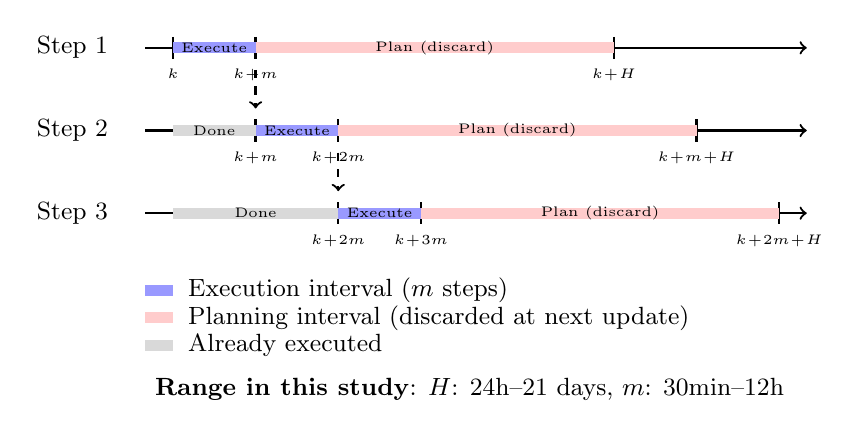
\begin{tikzpicture}[scale=0.7]
    % ステップ1
    \node[anchor=east] at (-0.5, 3) {\small Step 1};
    \draw[->, thick] (0,3) -- (12,3);
    \draw[thick] (0.5,3.2) -- (0.5,2.8) node[below] {\tiny $k$};
    \draw[thick] (2.0,3.2) -- (2.0,2.8) node[below] {\tiny $k\!+\!m$};
    \draw[thick] (8.5,3.2) -- (8.5,2.8) node[below] {\tiny $k\!+\!H$};
    \fill[blue!40] (0.5,2.9) rectangle (2.0,3.1);
    \fill[red!20] (2.0,2.9) rectangle (8.5,3.1);
    \node at (1.25,3) {\tiny Execute};
    \node at (5.25,3) {\tiny Plan (discard)};

    % ステップ2
    \node[anchor=east] at (-0.5, 1.5) {\small Step 2};
    \draw[->, thick] (0,1.5) -- (12,1.5);
    \draw[thick] (2.0,1.7) -- (2.0,1.3) node[below] {\tiny $k\!+\!m$};
    \draw[thick] (3.5,1.7) -- (3.5,1.3) node[below] {\tiny $k\!+\!2m$};
    \draw[thick] (10.0,1.7) -- (10.0,1.3) node[below] {\tiny $k\!+\!m\!+\!H$};
    \fill[gray!30] (0.5,1.4) rectangle (2.0,1.6);
    \fill[blue!40] (2.0,1.4) rectangle (3.5,1.6);
    \fill[red!20] (3.5,1.4) rectangle (10.0,1.6);
    \node at (1.25,1.5) {\tiny Done};
    \node at (2.75,1.5) {\tiny Execute};
    \node at (6.75,1.5) {\tiny Plan (discard)};

    % ステップ3
    \node[anchor=east] at (-0.5, 0) {\small Step 3};
    \draw[->, thick] (0,0) -- (12,0);
    \draw[thick] (3.5,0.2) -- (3.5,-0.2) node[below] {\tiny $k\!+\!2m$};
    \draw[thick] (5.0,0.2) -- (5.0,-0.2) node[below] {\tiny $k\!+\!3m$};
    \draw[thick] (11.5,0.2) -- (11.5,-0.2) node[below] {\tiny $k\!+\!2m\!+\!H$};
    \fill[gray!30] (0.5,-0.1) rectangle (3.5,0.1);
    \fill[blue!40] (3.5,-0.1) rectangle (5.0,0.1);
    \fill[red!20] (5.0,-0.1) rectangle (11.5,0.1);
    \node at (2,0) {\tiny Done};
    \node at (4.25,0) {\tiny Execute};
    \node at (8.25,0) {\tiny Plan (discard)};

    % 矢印(ステップ間の遷移)
    \draw[->, thick, dashed] (2.0, 2.6) -- (2.0, 1.9);
    \draw[->, thick, dashed] (3.5, 1.1) -- (3.5, 0.4);

    % 凡例(縦に並べて重なりを解消)
    \fill[blue!40] (0,-1.5) rectangle (0.5,-1.3);
    \node[anchor=west] at (0.6,-1.4) {\small Execution interval ($m$ steps)};
    \fill[red!20] (0,-2.0) rectangle (0.5,-1.8);
    \node[anchor=west] at (0.6,-1.9) {\small Planning interval (discarded at next update)};
    \fill[gray!30] (0,-2.5) rectangle (0.5,-2.3);
    \node[anchor=west] at (0.6,-2.4) {\small Already executed};

    % 本研究での範囲
    \node[anchor=west] at (0,-3.2) {\small \textbf{Range in this study}: $H$: 24h--21 days, $m$: 30min--12h};
\end{tikzpicture}
\caption{Conceptual diagram of the rolling horizon approach. A plan is formulated over the prediction horizon $H$, only the first $m$ steps are executed, and replanning is performed based on updated information. In this study, both $H$ and $m$ are varied for comparison.}
\label{fig:rolling_horizon}
\end{figure}

\section{システムモデルと定式化}

\subsection{用語の定義}

本論文で使用する主要な用語を以下に定義する.

\begin{itemize}
    \item \textbf{電力系統(系統)}:発電所から電力消費者(施設や家庭など)まで電力を供給するための送電・配電網の総称.本研究では,施設が電力会社から電力を購入する際の接続先を指す.
    \item \textbf{買電}:電力系統から電力を購入すること.その電力量を買電量 [kWh],瞬時電力を買電電力 [kW] と呼ぶ.
    \item \textbf{契約電力}:電力会社との契約で定める最大需要電力 [kW].高圧契約の場合,過去1年間の各月の最大需要電力(30分平均値)のうち最大のものが適用される.料金体系の詳細は3.3節で述べる.
    \item \textbf{SOC(State of Charge)}:蓄電池の充電残量を0〜100\%で表す指標.本研究ではkWh単位の残量$b^{\mathrm{F}}_{k}$を用いる.
    \item \textbf{出力抑制}:蓄電池が満充電かつ需要が少ない場合などに,PV発電可能量の一部をやむを得ず使用できず廃棄すること.
\end{itemize}

\subsection{対象システムの概要}

本研究では,2024年1月1日から同年12月31日までの365日間(2月29日を除く17,520ステップ,30分時間解像度)を対象期間とし,以下の仕様を持つシステムについてシミュレーションを行った.

\begin{itemize}
    \item \textbf{太陽光発電(PV)システム}:定格出力は250kWであり,パネルは南向き,設置角度40°で固定されている.
    \item \textbf{蓄電池システム}:蓄電池容量は本研究の比較軸の1つであり,0kWhから1720kWhの範囲で変化させて経済性を評価する.蓄電池の最大充電出力および最大放電出力はいずれも400kWである.初期SOCは容量の50\%とし,蓄電池の充放電効率はいずれも0.98(リチウムイオン電池の一般的な値)と設定した.
    \item \textbf{系統電力}:本研究では,北海道電力の固定料金プランおよびJEPX(日本卸電力取引所)のスポット価格に連動する市場価格連動プランの2種類の料金体系を比較検討する.詳細は3.3節で述べる.
\end{itemize}

システム構成の概念図をFig.\ref{fig:system_config}に示す.

\begin{figure}[H]
\centering
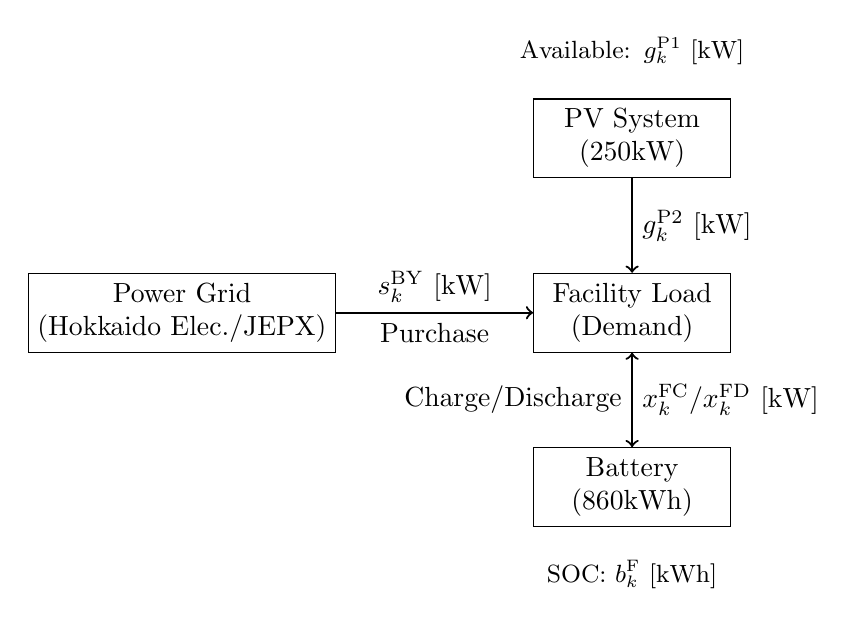
\begin{tikzpicture}[
    node distance=1.5cm,
    block/.style={rectangle, draw, minimum width=2.5cm, minimum height=1cm, align=center},
    arrow/.style={->, thick},
    darrow/.style={<->, thick}
]
% ノード定義
\node[block] (grid) {Power Grid\\(Hokkaido Elec./JEPX)};
\node[block, right=2.5cm of grid] (load) {Facility Load\\(Demand)};
\node[block, above=1.2cm of load] (pv) {PV System\\(250kW)};
\node[block, below=1.2cm of load] (battery) {Battery\\(860kWh)};

% 矢印
\draw[arrow] (grid) -- node[above] {$s^{\mathrm{BY}}_k$ [kW]} node[below] {Purchase} (load);
\draw[arrow] (pv) -- node[right] {$g^{\mathrm{P2}}_k$ [kW]} (load);
\draw[darrow] (battery) -- node[right] {$x^{\mathrm{FC}}_k / x^{\mathrm{FD}}_k$ [kW]} node[left] {Charge/Discharge} (load);

% 注釈
\node[below=0.3cm of battery, text width=3cm, align=center, font=\small] {SOC: $b^{\mathrm{F}}_k$ [kWh]};
\node[above=0.3cm of pv, text width=4cm, align=center, font=\small] {Available: $g^{\mathrm{P1}}_k$ [kW]};
\end{tikzpicture}
\caption{Schematic of the system configuration. Facility demand is met by purchased power from the grid, PV generation, and battery charge/discharge.}
\label{fig:system_config}
\end{figure}

\subsection{料金体系}

本研究で比較検討する2種類の料金体系について説明する.日本の高圧電力契約における電気料金は,\textbf{基本料金}(契約電力に基づく固定費)と\textbf{電力量料金}(実際の使用電力量に応じた従量費)の合計で構成される:
\begin{equation}
\text{電気料金} = \text{基本料金} + \text{電力量料金}
\end{equation}

\subsubsection{北海道電力基本プラン(高圧電力,一般料金)}

北海道電力の料金体系をTable~\ref{tab:hokkaido_tariff}に示す.

\begin{table}[H]
\centering
\caption{Tariff structure of Hokkaido Electric Power (effective April 1, 2024)}
\label{tab:hokkaido_tariff}
\begin{tabular}{lc}
\toprule
Item & Unit Price \\
\midrule
Basic charge & 2,829.60 JPY/kW \\
Energy charge & 21.51 JPY/kWh \\
Renewable levy & 3.98 JPY/kWh \\
\bottomrule
\end{tabular}
\end{table}

\textbf{基本料金の計算式:}
\begin{equation}
C_{\mathrm{basic}} = P_{\mathrm{contract}} \times 2829.60 \times 0.85 \times 12 \quad \text{[円/年]}
\end{equation}

ここで,$P_{\mathrm{contract}}$は契約電力であり,過去1年間の各月の最大需要電力のうち,最も大きい値を適用する.2829.60は基本料金単価(円/kW),0.85は力率割引係数,12は年間月数である.本シミュレーションでは,1年間の運用結果から得られた最大買電電力を$P_{\mathrm{contract}}$として事後的に計算している.

\textbf{電力量料金の計算式:}
\begin{equation}
C_{\mathrm{energy}} = E_{\mathrm{month}} \times (21.51 + F_{\mathrm{adj}}(m) + 3.98) \quad \text{[円/月]}
\end{equation}

ここで,$E_{\mathrm{month}}$は月間電力使用量 [kWh],21.51は電力量料金単価(円/kWh),$F_{\mathrm{adj}}(m)$は$m$月($m \in \{1,2,\dots,12\}$)の燃料費調整額(円/kWh),3.98は再生可能エネルギー発電促進賦課金(円/kWh)である.

2024年の月別燃料費調整額をTable~\ref{tab:fuel_adjustment}に示す.

\begin{table}[H]
\centering
\caption{Monthly fuel cost adjustment charges in 2024 (Hokkaido Electric, high-voltage)}
\label{tab:fuel_adjustment}
\begin{tabular}{cc}
\toprule
Month & Fuel Adj. [JPY/kWh] \\
\midrule
Jan & $-8.76$ \\
Feb & $-8.59$ \\
Mar & $-8.56$ \\
Apr & $-8.85$ \\
May & $-9.02$ \\
Jun & $-7.47$ \\
Jul & $-5.69$ \\
Aug & $-5.69$ \\
Sep & $-9.60$ \\
Oct & $-9.47$ \\
Nov & $-8.06$ \\
Dec & $-5.83$ \\
\bottomrule
\end{tabular}
\end{table}

\subsubsection{市場価格連動プラン}

市場価格連動プランでは,電力量料金がJEPX(日本卸電力取引所)のスポット価格に連動する.

\textbf{電力量料金の計算式:}
\begin{equation}
C_{\mathrm{energy}} = E_{\mathrm{month}} \times (P_{\mathrm{JEPX}}(t) + 3.98) \quad \text{[円/月]}
\end{equation}

ここで,$P_{\mathrm{JEPX}}(t)$は時刻 $t$ のJEPXスポット価格(円/kWh),3.98は再生可能エネルギー発電促進賦課金(円/kWh)である.基本料金は北海道電力と同額とする.

\subsection{運用制約条件}

システム運用における最適化計算では,以下の物理的および制度的制約を課した.

\begin{itemize}
    \item \textbf{電力需給平衡}:各タイムステップにおいて,供給電力(PV発電,買電,蓄電池放電)の総和は,需要電力(施設需要,蓄電池充電)の総和と常に一致しなければならない.
    \item \textbf{蓄電池運用制約}:蓄電池の劣化抑制および安全性を考慮し,SOCの運用範囲は定格容量の5\%から95\%に制限した(容量860kWhの場合,43kWh以上817kWh以下).また,充放電電力は最大出力(400kW)以下とし,充電と放電の同時実行を禁止する排他制御も行う.
    \item \textbf{系統への電力逆流禁止}:PV発電の余剰電力が生じた場合でも,系統への電力逆流(電力の送り返し)は行わず,システム内で消費または出力抑制するものとした.
\end{itemize}


\subsection{数理モデルの定式化}

本節で使用する記号をTable~\ref{tab:symbols}にまとめる.

\begin{table}[H]
\centering
\caption{List of symbols}
\label{tab:symbols}
\begin{tabular}{clc}
\toprule
Symbol & Description & Unit \\
\midrule
\multicolumn{3}{l}{\textbf{Decision Variables}} \\
$s^{\mathrm{BY}}_{k}$ & Purchased power at step $k$ & kW \\
$s^{\mathrm{BY}}_{\mathrm{MAX}}$ & Max purchased power in horizon & kW \\
$x^{\mathrm{FC1}}_{k}$, $x^{\mathrm{FC2}}_{k}$ & Charge power (before/after conv.) & kW \\
$x^{\mathrm{FD1}}_{k}$, $x^{\mathrm{FD2}}_{k}$ & Discharge power (before/after conv.) & kW \\
$b^{\mathrm{F}}_{k}$ & Battery SOC & kWh \\
$z_{k}$ & Charge/discharge mode (1:charge, 0:discharge) & -- \\
$g^{\mathrm{P2}}_{k}$ & Actual PV generation used & kW \\
\midrule
\multicolumn{3}{l}{\textbf{Known Parameters}} \\
$g^{\mathrm{P1}}_{k}$ & Available PV generation & kW \\
$d_{k}$ & Demand power & kW \\
$p^{\mathrm{BY}}_{k}$ & Energy price & JPY/kWh \\
\midrule
\multicolumn{3}{l}{\textbf{Constants}} \\
$H$ & Prediction horizon & steps \\
$\Delta t$ & Time per step (= 0.5) & h \\
$\eta$ & Charge/discharge efficiency (= 0.98) & -- \\
$C_{\mathrm{bat}}$ & Battery rated capacity & kWh \\
$P^{\mathrm{FC}}_{\mathrm{max}}$, $P^{\mathrm{FD}}_{\mathrm{max}}$ & Max charge/discharge power (= 400) & kW \\
$C_{\mathrm{cap}}$ & Annual basic charge rate & JPY/kW \\
$w_{\mathrm{basic}}$ & Basic charge weight coefficient & JPY/kW \\
$M$ & Big-M constant (= $10^6$) & -- \\
\bottomrule
\end{tabular}
\end{table}

\subsubsection{決定変数}

最適化問題における決定変数はTable~\ref{tab:symbols}の通りである.連続変数は非負とし,添字$k$は時刻ステップ($k = 0, 1, \ldots, H-1$)を表す.

既知パラメータとして,PV発電可能量$g^{\mathrm{P1}}_{k}$および需要電力$d_{k}$を与える.出力抑制を許容し,$g^{\mathrm{P2}}_{k} \leq g^{\mathrm{P1}}_{k}$とする.

\subsubsection{目的関数}

日本の高圧電力契約では,電気料金は以下の2つから構成される:
\begin{itemize}
    \item \textbf{基本料金}:契約電力(過去1年間の最大需要電力)に基づく固定費
    \item \textbf{電力量料金}:実際の使用電力量に応じた従量費
\end{itemize}

\noindent
目的関数は,予測期間$H$における電気料金(基本料金相当額および電力量料金)の総和とし,これを最小化する.

\begin{equation}
\text{Minimize} \quad J = \underbrace{w_{\mathrm{basic}} \cdot s^{\mathrm{BY}}_{\mathrm{MAX}}}_{\text{基本料金相当額}} + \underbrace{\sum_{k=0}^{H-1} p^{\mathrm{BY}}_{k} \cdot s^{\mathrm{BY}}_{k} \cdot \Delta t}_{\text{電力量料金}}
\label{eq:objective}
\end{equation}

\noindent
\textbf{目的関数の設計に関する考察:}
本研究の目的関数は各予測期間$H$内のコスト最小化であり,年間電気料金を直接最小化するものではない.契約電力は年間の最大需要電力で決まる大域的な指標であるため,本来は全17,520ステップを一括して最適化すべきである.しかし,現実的な計算負荷の制約に加え,予測誤差への柔軟な対応やフィードバック的な運用を実現するため,本研究ではローリング計画法を採用した.

この手法では,各ステップの最適化において考慮されるのは予測期間$H$内のピーク電力のみである.そのため,期間外の需要ピークや将来の価格変動を完全に予見できず,結果として年間契約電力の削減効果が限定的になる可能性がある.

ここで,$p^{\mathrm{BY}}_{k}$は時刻$k$における買電電力量単価(北海道電力基本プランでは固定値,市場連動プランではJEPXスポット価格)[円/kWh],$w_{\mathrm{basic}}$は基本料金に関する重み係数 [円/kW]である.

基本料金は本来,年間の最大需要電力に基づいて決定されるが,本手法では予測期間が限定的であるため,年間の基本料金単価を時間按分した値をペナルティ項として導入した.重み係数$w_{\mathrm{basic}}$は式(\ref{eq:weight_basic})により算出される.

\begin{equation}
w_{\mathrm{basic}} = C_{\mathrm{cap}} \times \frac{H \cdot \Delta t}{8760}
\label{eq:weight_basic}
\end{equation}

ここで,8760は1年間の時間数($365 \times 24$時間)であり,年間基本料金を予測期間の長さに応じて按分している.

ただし,$C_{\mathrm{cap}}$は年間基本料金単価であり,表\ref{tab:hokkaido_tariff}の料金単価に基づき以下のように算出される:
\begin{equation}
C_{\mathrm{cap}} = 2,829.60 \times 0.85 \times 12 \quad \text{[円/kW]}
\end{equation}
ここで,2,829.60円/kWは月額基本料金単価,0.85は力率割引係数(力率85\%以上で適用),12は年間月数である.この項の導入により,各予測期間における買電電力の最大値の抑制を図り,間接的に年間契約電力の低減を指向する.

\noindent
\textbf{注}:本手法は「局所的な最大値の抑制」を通じて「大域的な最大値(年間契約電力)」を間接的に制御する近似であり,その限界については考察(\ref{sec:wbasic_limitation}節)で詳述する.

\subsubsection{制約条件}

システムの物理的特性および運用上の要請に基づき,以下の制約条件を課す.

\noindent
\textbf{(1) 電力需給バランス制約}

各時刻において,供給と需要は一致しなければならない.
\begin{equation}
g^{\mathrm{P2}}_{k} + s^{\mathrm{BY}}_{k} + x^{\mathrm{FD2}}_{k} = d_{k} + x^{\mathrm{FC1}}_{k}, \quad \forall k
\label{eq:balance}
\end{equation}

蓄電池の充放電電力は変換効率$\eta = 0.98$を介して以下の関係にある.
\begin{align}
x^{\mathrm{FC2}}_{k} &= \eta \cdot x^{\mathrm{FC1}}_{k} \label{eq:fc_eff} \\
x^{\mathrm{FD2}}_{k} &= \eta \cdot x^{\mathrm{FD1}}_{k} \label{eq:fd_eff}
\end{align}

ここで,$x^{\mathrm{FC1}}_{k}$は蓄電池への入力電力(変換前),$x^{\mathrm{FC2}}_{k}$は蓄電池に実際に蓄積される電力(変換後)を表す.放電についても同様に,$x^{\mathrm{FD1}}_{k}$は蓄電池から取り出す電力(変換前),$x^{\mathrm{FD2}}_{k}$は蓄電池由来の,負荷で利用可能な電力(変換後)である.

\noindent
\textbf{(2) 蓄電池状態遷移および容量制約}

蓄電池のSOC推移は次式で記述される.
\begin{equation}
b^{\mathrm{F}}_{k+1} = b^{\mathrm{F}}_{k} + (x^{\mathrm{FC2}}_{k} - x^{\mathrm{FD1}}_{k}) \cdot \Delta t
\label{eq:soc_update}
\end{equation}

また,過充電・過放電防止のため,運用範囲を定格容量$C_{\mathrm{bat}}$の5\%〜95\%に制限する.
\begin{equation}
0.05 \cdot C_{\mathrm{bat}} \leq b^{\mathrm{F}}_{k} \leq 0.95 \cdot C_{\mathrm{bat}}, \quad \forall k
\label{eq:soc_limit}
\end{equation}

\noindent
\textbf{(3) 充放電排他および出力制約}

充電と放電の同時実行を物理的に排除するため,二値変数$z_{k}$を用いた以下の制約(Big-M法)を設ける.
\begin{align}
x^{\mathrm{FC1}}_{k} &\leq M \cdot z_{k}, \quad \forall k \label{eq:bigm_fc} \\
x^{\mathrm{FD1}}_{k} &\leq M \cdot (1 - z_{k}), \quad \forall k \label{eq:bigm_fd}
\end{align}

ここで,$M$は十分大きな定数($M = 10^6$)である.また,充放電出力の上限として以下を課す.
\begin{align}
x^{\mathrm{FC2}}_{k} &\leq P^{\mathrm{FC}}_{\mathrm{max}}, \quad \forall k \label{eq:fc_limit} \\
x^{\mathrm{FD1}}_{k} &\leq P^{\mathrm{FD}}_{\mathrm{max}}, \quad \forall k \label{eq:fd_limit}
\end{align}

本研究では$P^{\mathrm{FC}}_{\mathrm{max}} = P^{\mathrm{FD}}_{\mathrm{max}} = 400$\,kWとした.

\noindent
\textbf{(4) PV出力制約}

実際に使用するPV発電量は発電可能量を超えない.
\begin{equation}
g^{\mathrm{P2}}_{k} \leq g^{\mathrm{P1}}_{k}, \quad \forall k
\label{eq:pv_limit}
\end{equation}

\noindent
\textbf{(5) 契約電力制約}

予測期間内のすべての時刻において,買電電力は$s^{\mathrm{BY}}_{\mathrm{MAX}}$以下でなければならない.
\begin{equation}
s^{\mathrm{BY}}_{k} \leq s^{\mathrm{BY}}_{\mathrm{MAX}}, \quad \forall k
\label{eq:contract}
\end{equation}

\section{実験設定}

\subsection{使用データ}

本シミュレーションでは,以下の実測データおよび市場価格データを使用した.

\begin{itemize}
    \item \textbf{対象期間}:2024年1月1日から同年12月31日までの365日間.2024年は閏年であるが,365日間(1年間)の統一的な解析のため2月29日を除外した全17,520ステップ(30分時間分解能)を解析対象とした.
    \item \textbf{電力需要およびPV発電量}:北海道十勝地方の対象施設における実測値(30分積算値)を使用した.
    \item \textbf{電力市場価格}:一般社団法人日本卸電力取引所(JEPX)が公開する北海道エリアのスポット市場価格(30分値)を採用した.
\end{itemize}

\subsection{データ前処理}

取得データは30分間の積算電力量$E_{30\mathrm{min}}$\,[kWh]であるため,最適化計算の入力とするにあたり,以下の関係式を用いて平均電力$P_{\mathrm{avg}}$\,[kW]に換算した.
\begin{equation}
P_{\mathrm{avg}} = \frac{E_{30\mathrm{min}}}{0.5}
\label{eq:power_conversion}
\end{equation}

なお,目的関数の電力量料金項の算出に際しては,決定変数(電力\,[kW])に時間刻み$\Delta t = 0.5$\,[h]を乗じることで,再び電力量\,[kWh]ベースに換算して評価を行っている.

\subsection{計算環境と実装}

アルゴリズムの実装にはPython 3.xを使用し,混合整数計画問題(MILP)のソルバーにはSCIPのPythonインターフェースであるPySCIPOptを採用した.数値計算およびデータ処理にはpandas,numpyライブラリを,結果の可視化にはmatplotlibをそれぞれ用いた.

\subsection{最適化パラメータ}

ローリング計画法における予測期間$H$は,以下のケースについて比較検証を行った:短期予測として$H=48$(24時間),$H=96$(48時間),$H=120$(60時間),$H=144$(72時間)の4ケース,長期予測として$H=192$(4日間),$H=384$(8日間),$H=672$(14日間),$H=1008$(21日間)の4ケースである.再計画間隔$m$は基本的に$m=1$(30分ごとに再計画)とし,長期予測では計算負荷軽減のため$m=8$(4時間)や$m=24$(12時間)も検討した.

\section{結果と考察}

本章では,まず5.1節でシステムの基本的な運用パターンを示した後,5.2節以降で3つの比較軸(蓄電池容量・予測期間・再計画間隔)に沿って詳細な結果を報告する.いずれの結果も特定の条件下での結論であり,条件によって最適なプランが異なる点に留意されたい.

\subsection{システムの運用特性と季節変動分析}

需給条件の異なる代表的な日における運用挙動をFig.\ref{fig:battery_operation}およびFig.\ref{fig:battery_operation_low}に示す.これらの図は蓄電池容量860kWh,北海道電力基本プランの条件下での結果である.

\noindent
\textbf{高需要日}:6月2日(需要2,436kWh,PV発電1,433kWh)と6月24日(需要2,461kWh,PV発電237kWh)を比較する.PV発電が豊富な6月2日は,昼間の余剰電力を蓄電し夜間に放電することで,買電量を1,275kWh(需要の52.4\%)に抑制した.一方,PV発電が少ない6月24日は買電量が2,080kWh(需要の84.5\%)に増加し,買電依存度の差は1.6倍となった.

\noindent
\textbf{低需要日}:2月5日(需要1,284kWh,PV発電1,019kWh)と1月22日(需要1,298kWh,PV発電281kWh)を比較する.PV発電が豊富な2月5日は買電量が270kWh(需要の21.0\%)まで減少し,高い自給率を実現した.一方,PV発電が少ない1月22日は買電量が862kWh(需要の66.4\%)となり,買電依存度の差は3.2倍に達した.この結果から,低需要日においてはPV発電量の多さ・少なさが買電量に与える影響が高需要日よりも顕著であることが確認された.

\begin{figure}[H]
\centering
\includegraphics[width=\textwidth]{../png/soc860/daily_battery_pattern.png}
\caption{Operation patterns on high-demand days (demand $\approx$ 2,450\,kWh). Top: high PV generation day (June 2, 2024, PV 1,433\,kWh). Bottom: low PV generation day (June 24, 2024, PV 237\,kWh).}
\label{fig:battery_operation}
\end{figure}

\begin{figure}[H]
\centering
\includegraphics[width=\textwidth]{../png/soc860/daily_battery_pattern_low_demand.png}
\caption{Operation patterns on low-demand days (demand $\approx$ 1,290\,kWh). Top: high PV generation day (Feb. 5, 2024, PV 1,019\,kWh). Bottom: low PV generation day (Jan. 22, 2024, PV 281\,kWh).}
\label{fig:battery_operation_low}
\end{figure}

また,Fig.\ref{fig:battery_operation}やFig.\ref{fig:battery_operation_low}において買電電力が一定値を維持する挙動が観察されるが,これは式(\ref{eq:objective})で導入した基本料金項の影響である.契約電力の増大を回避しつつ,蓄電池の充放電で需給調整を行う最適制御が機能していることを示す.

本運用パターンに加え,季節変動や市場価格特性がシステムに与える影響を以下で詳細に分析する.なお,本節の以下の分析は\textbf{予測期間48時間,蓄電池860kWh,再計画間隔30分($m=1$)}という条件下での結果である.

\subsubsection{季節別の蓄電池効果}

蓄電池860kWhの運用データを月別に分析した結果をTable~\ref{tab:monthly_analysis}に示す.ここで,買電抑制率(Reduction)は次式で算出した値であり,蓄電池によって買電の最大電力がどの程度抑制されたかを示す.
\begin{equation}
\text{Reduction} = \frac{\text{需要の最大電力(Peak Demand)} - \text{買電の最大電力(Peak Purchase)}}{\text{需要の最大電力}} \times 100
\end{equation}

\begin{table}[H]
\centering
\small
\caption{Monthly energy statistics and battery effect}
\label{tab:monthly_analysis}
\resizebox{\textwidth}{!}{%
\begin{tabular}{lrrrrrr}
\toprule
Month & Demand [MWh] & PV [MWh] & Purchase [MWh] & Peak Demand [kW] & Peak Purchase [kW] & Reduction [\%] \\
\midrule
Jan & 40.2 & 20.9 & 19.7 & 130.0 & 41.0 & 68.5 \\
Feb & 36.7 & 25.3 & 12.3 & 150.0 & 29.0 & 80.7 \\
Mar & 49.0 & 32.4 & 16.8 & 154.0 & 36.2 & 76.5 \\
Apr & 54.9 & 26.6 & 29.0 & 220.0 & 64.0 & 70.9 \\
May & 66.6 & 27.1 & 39.9 & 204.0 & 80.4 & 60.6 \\
Jun & 77.6 & 24.8 & 53.3 & 246.0 & 121.8 & 50.5 \\
Jul & 111.2 & 25.6 & 86.2 & 260.0 & 154.9 & 40.4 \\
Aug & 118.2 & 18.8 & 99.8 & 264.0 & 166.8 & 36.8 \\
Sep & 90.9 & 24.9 & 66.7 & 242.0 & 139.0 & 42.6 \\
Oct & 72.5 & 22.0 & 50.9 & 218.0 & 115.5 & 47.0 \\
Nov & 49.9 & 19.5 & 30.8 & 144.0 & 61.0 & 57.6 \\
Dec & 45.3 & 19.8 & 25.8 & 150.0 & 43.5 & 71.0 \\
\midrule
Annual & 813.0 & 287.6 & 531.4 & 264.0 & 166.8 & -- \\
\bottomrule
\end{tabular}%
}
\end{table}

Fig.\ref{fig:price_charge_scatter}に,JEPX価格と充放電量の関係を散布図として示す.この図は市場価格連動プランにおいて,最適化アルゴリズムがどのような価格帯で充放電を行っているか,価格に応じた充放電パターンを可視化したものである.

\begin{figure}[H]
\centering
\includegraphics[width=\textwidth]{../png/thesis_figures/price_charge_scatter.png}
\caption{Relationship between JEPX price and charge/discharge power (market-linked plan, battery 860\,kWh). Left: charging power. Right: discharging power. Colors represent months. A clear policy of charging at low prices and discharging at high prices is observed.}
\label{fig:price_charge_scatter}
\end{figure}

Fig.\ref{fig:price_charge_bar}に,価格帯別の平均充放電電力を示す.これにより,最適化アルゴリズムの価格応答特性が定量的に把握できる.

\begin{figure}[H]
\centering
\includegraphics[width=0.9\textwidth]{../png/thesis_figures/price_charge_bar.png}
\caption{Average charge/discharge power by price range (market-linked plan). Charging is active in the low-price range (0--10\,JPY/kWh), while discharging increases in the high-price range (above 25\,JPY/kWh).}
\label{fig:price_charge_bar}
\end{figure}

\noindent
月別分析から,蓄電池効果の季節依存性について重要な知見が得られた.

冬季(12--2月)は蓄電池効果が最も高く,買電抑制率68.5〜80.7\%を達成した.この理由は,冬季の需要122.2MWhに対しPV発電65.9MWh(需要の54\%)が確保されており,蓄電池容量860kWhが需要に対して相対的に大きいためである.特に2月は買電抑制率80.7\%と最高値を記録した.一方,夏季(6--8月)は蓄電池効果が最小となり,買電抑制率は36.8〜50.5\%に留まった.夏季は需要307.0MWhと年間最大である一方,PV発電は69.3MWh(需要の23\%)に過ぎないためである.特に8月は需要118.2MWhに対しPV発電18.8MWhと最も需給バランスが悪く,蓄電池容量860kWhをもってしても買電の最大電力を十分に抑制することができなかった.

PV発電量の季節パターンについては,3月が32.4MWhで最大,8月が18.8MWhで最小となった.夏季は需要が最大となる一方でPV発電量が相対的に低いため,需給バランスの観点から最も厳しい季節である.

契約電力の決定要因については,年間の買電最大電力が8月に発生(166.8kW)した点が注目される.夏季は買電抑制率が低く,かつ需要の最大電力が大きい(8月:264.0kW)ため,蓄電池による抑制後もなお買電最大電力が高くなる.すなわち,夏季の高需要期が年間を通じた契約電力を決定づける「ボトルネック」となっている.

蓄電池の劣化に関しては,年間推定218サイクル(月平均18サイクル)であった.なお,1サイクルとは蓄電池容量相当の電力量を充放電する単位を指し,部分的な充放電は累積して換算する.

Fig.\ref{fig:monthly_analysis}に月別エネルギー量と買電抑制率のグラフを示す.

\begin{figure}[H]
    \centering
    \includegraphics[width=0.95\textwidth]{../png/soc860/monthly_analysis.png}
    \caption{Monthly energy and battery effect analysis. ``PV self-consumption ratio'' in the bottom-left graph indicates the proportion of PV generation directly consumed by demand. ``Battery discharge contribution'' is the ratio of battery discharge to total demand. The ``purchase reduction rate'' in the bottom-right graph is calculated as $(\text{peak demand} - \text{peak purchase}) / \text{peak demand} \times 100$.}
    \label{fig:monthly_analysis}
\end{figure}

\subsubsection{市場価格(JEPX)の季節変動特性}

JEPXスポット価格の月別統計をTable~\ref{tab:price_monthly}に示す.表中のMean,Median,Min,Maxはそれぞれ平均,中央値,最小値,最大値を表す.「$>$北電率($>$Hokkaido)」は市場価格が北海道電力基本プランの電力量料金(21.51円/kWh)を上回る時間帯の割合を示す.

\begin{table}[H]
\centering
\small
\caption{Monthly market price statistics}
\label{tab:price_monthly}
\resizebox{\textwidth}{!}{%
\begin{tabular}{lrrrrrr}
\toprule
Month & Mean [JPY/kWh] & Median [JPY/kWh] & Min [JPY/kWh] & Max [JPY/kWh] & $>$Hokkaido [\%] & High-price Count \\
\midrule
Jan & 14.07 & 13.79 & 3.99 & 23.10 & 0.4 & 0 \\
Feb & 13.42 & 13.00 & 3.99 & 25.22 & 1.9 & 2 \\
Mar & 15.94 & 15.79 & 3.99 & 40.57 & 11.4 & 16 \\
Apr & 14.30 & 15.52 & 3.99 & 23.98 & 4.4 & 0 \\
May & 15.67 & 16.03 & 3.99 & 25.88 & 14.0 & 4 \\
Jun & 16.72 & 16.52 & 3.99 & 25.75 & 15.4 & 12 \\
Jul & 18.39 & 17.48 & 3.99 & 33.98 & 26.1 & 124 \\
Aug & 19.15 & 19.62 & 8.99 & 25.31 & 32.8 & 60 \\
Sep & 19.27 & 17.98 & 3.99 & 53.63 & 30.3 & 104 \\
Oct & 18.75 & 18.05 & 3.99 & 42.98 & 37.6 & 30 \\
Nov & 18.78 & 18.45 & 6.98 & 25.30 & 29.4 & 30 \\
Dec & 17.70 & 18.09 & 4.00 & 26.98 & 16.4 & 18 \\
\bottomrule
\end{tabular}%
}
\end{table}

\noindent
「高価格回数(High-price Count)」は25円/kWh以上の価格が発生した30分コマ数を示す.年間最高価格53.63円/kWhは2024年9月20日9:00に発生した.

市場価格分析から,JEPX価格の特性と料金プラン選択への示唆が得られた.

まず,市場価格の年間平均は16.87円/kWhであり,北海道電力基本プラン(21.51円/kWh)より21.6\%安い.この単純比較からは市場価格連動プランが有利に見えるが,この比較は買電タイミングを考慮していない点に注意が必要である.実際,年間17,520コマのうち3,236コマ(18.5\%)で市場価格が21.51円/kWhを超過しており,市場価格が北電電力量料金を超過する割合は秋季(9--11月)で32.5\%と最も高く,冬季(12--2月)は6.4\%と最も低い.

高価格帯の発生パターンを詳細に分析すると,25円/kWh以上の高価格は年間400回(2.3\%)発生し,その大部分が7月(124回),9月(104回),8月(60回)に集中している.時間帯別には,25円/kWh以上の高価格は9:00--14:00に集中しており,高価格帯の発生が上位5時間帯に57.5\%集中している.この時間帯は需要も高いため,市場価格連動プランでは高価格での買電が避けられない構造となっている.

時間帯別価格パターンについては,深夜(0:00--2:00)は平均11--12円/kWh,昼間(11:00--14:00)は平均20--21円/kWhと,約2倍の価格差が存在する.市場価格連動プランはこの価格差を利用した時間シフトが理論上可能であるが,需要パターンとの制約により完全な活用は困難である.

\subsection{蓄電池容量と料金プランの経済性評価}

本節では,予測期間$H=96$(48時間),再計画間隔$m=1$(30分)の条件下において,\textbf{蓄電池容量}を変化させた際の経済性を比較する(Fig.\ref{fig:axis_battery}).なお,この条件は複数の検証ケースのうちの1つであり,予測期間が異なれば結論が変わりうる点に留意されたい(5.4節,5.5節で詳述).

\begin{figure}[H]
\centering
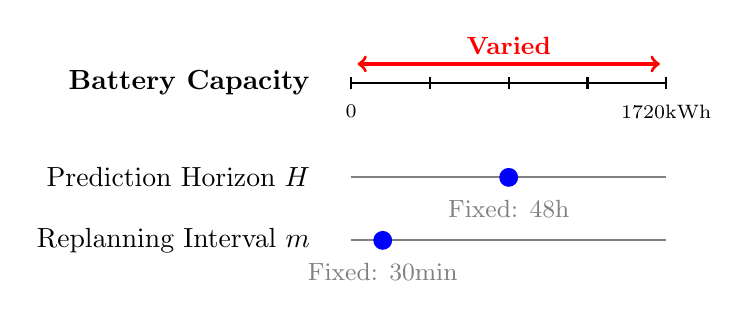
\begin{tikzpicture}[scale=0.8]
    % 蓄電池容量(変化)
    \node[anchor=east] at (-0.5,0) {\textbf{Battery Capacity}};
    \draw[thick] (0,0) -- (5,0);
    \foreach \x/\label in {0/0, 1.25/430, 2.5/860, 3.75/1290, 5/1720} {
        \draw[thick] (\x,-0.1) -- (\x,0.1);
    }
    \node[below] at (0,-0.2) {\scriptsize 0};
    \node[below] at (5,-0.2) {\scriptsize 1720kWh};
    \draw[red, very thick, <->] (0.1,0.3) -- (4.9,0.3);
    \node[red, above] at (2.5,0.3) {\small \textbf{Varied}};

    % 予測期間(固定)
    \node[anchor=east] at (-0.5,-1.5) {Prediction Horizon $H$};
    \draw[gray, thick] (0,-1.5) -- (5,-1.5);
    \fill[blue] (2.5,-1.5) circle (0.15);
    \node[below, gray] at (2.5,-1.7) {\small Fixed: 48h};

    % 再計画間隔(固定)
    \node[anchor=east] at (-0.5,-2.5) {Replanning Interval $m$};
    \draw[gray, thick] (0,-2.5) -- (5,-2.5);
    \fill[blue] (0.5,-2.5) circle (0.15);
    \node[below, gray] at (0.5,-2.7) {\small Fixed: 30min};
\end{tikzpicture}
\caption{Comparison axis of this section: battery capacity is varied from 0 to 1720\,kWh, while the prediction horizon and replanning interval are fixed.}
\label{fig:axis_battery}
\end{figure}

\subsubsection{蓄電池容量による経済性の変化}

蓄電池容量ごとの年間コスト比較をTable~\ref{tab:capacity_plan_comparison}およびTable~\ref{tab:optimal_comparison}に示す.

\begin{table}[H]
\centering
\caption{Annual cost comparison by battery capacity (both plans, $H=96$, $m=1$)}
\label{tab:capacity_plan_comparison}
\begin{tabular}{rrrrl}
\toprule
Capacity [kWh] & Hokkaido [JPY] & Market [JPY] & Diff. [JPY] & Cheaper Plan \\
\midrule
0 & 18,101,486 & 17,422,732 & $+678,754$ & Market \\
215 & 15,585,445 & 14,787,091 & $+798,354$ & Market \\
430 & 14,941,626 & 14,613,390 & $+328,236$ & Market \\
540 & 14,731,394 & 14,859,816 & $-128,422$ & Hokkaido \\
645 & 14,561,085 & 14,858,066 & $-296,981$ & Hokkaido \\
860 & 14,343,827 & 15,023,532 & $-679,705$ & Hokkaido \\
1290 & 14,074,455 & 15,125,066 & $-1,050,611$ & Hokkaido \\
1720 & 14,072,576 & 15,290,495 & $-1,217,919$ & Hokkaido \\
\bottomrule
\end{tabular}
\end{table}

\noindent
差額は「北電基本 $-$ 市場連動」を示す.正の値は市場連動プランが安価,負の値は北電基本プランが安価であることを意味する.

\noindent
\textbf{本条件下($H=96$,$m=1$)での料金プラン経済性}:蓄電池容量430kWh以下では市場価格連動プランが有利であるが,540kWh以上では北海道電力基本プランが有利となり,プラン優位性が逆転する.ただし,この結論は予測期間に依存し,長期予測では結果が変わる(5.4節,5.5節で詳述).

各料金プランにとって最適な蓄電池容量での比較をTable~\ref{tab:optimal_comparison}に示す.

\begin{table}[H]
\centering
\caption{Annual cost comparison at the lowest-cost capacity for each plan}
\label{tab:optimal_comparison}
\begin{tabular}{llrr}
\toprule
Pricing Plan & Lowest-cost Capacity & Annual Cost [JPY] & Contract Power [kW] \\
\midrule
Market-linked & 430 kWh & 14,613,390 & 201.40 \\
Hokkaido Electric & 1720 kWh & 14,072,576 & 157.40 \\
\midrule
\multicolumn{2}{l}{\textbf{Difference}} & \multicolumn{2}{l}{\textbf{540,814 JPY (Hokkaido cheaper)}} \\
\bottomrule
\end{tabular}
\end{table}

\noindent
\textbf{コスト最小容量での比較}:検討した蓄電池容量(0~1720kWh)の範囲で各プランのコストが最小となる容量(市場連動:430kWh,北電基本:1720kWh)を比較すると,北電基本プランが年間約54万円安価である.なお,本比較は離散的な容量設定に基づく.

\subsubsection{契約電力と運用特性の違い}

両プランの蓄電池容量別詳細比較をTable~\ref{tab:capacity_comparison_detail}およびTable~\ref{tab:capacity_comparison_market_detail}に示す.表中の「PV利用率」は「実際に使用したPV発電量 $\div$ PV発電可能量 $\times$ 100[\%]」で定義される.蓄電池容量が少ない場合,PV余剰電力をうまく活用できず出力抑制が発生するため100\%未満となる.

\begin{table}[H]
\centering
\caption{Detailed comparison by battery capacity (Hokkaido Electric basic plan)}
\label{tab:capacity_comparison_detail}
\resizebox{\textwidth}{!}{%
\begin{tabular}{rrrrrr}
\toprule
Capacity [kWh] & Contract Power [kW] & Purchase [kWh] & PV Util. [\%] & Annual Cost [JPY] & Cost Diff. [JPY] \\
\midrule
0 & 262.00 & 590,587 & 78.01 & 18,101,486 & - \\
215 & 198.01 & 551,647 & 92.43 & 15,585,445 & $-2,516,041$ \\
430 & 185.50 & 535,043 & 98.41 & 14,941,626 & $-3,159,860$ \\
540 & 179.76 & 532,389 & 99.46 & 14,731,394 & $-3,370,092$ \\
645 & 174.36 & 531,536 & 99.86 & 14,561,085 & $-3,540,401$ \\
860 & 166.83 & 531,528 & 100.0 & 14,343,827 & $-3,757,659$ \\
1290 & 157.40 & 531,672 & 100.0 & 14,074,455 & $-4,027,031$ \\
1720 & 157.40 & 531,553 & 100.0 & 14,072,576 & $-4,028,910$ \\
\bottomrule
\end{tabular}%
}
\end{table}

\begin{table}[H]
\centering
\caption{Detailed comparison by battery capacity (market-linked plan)}
\label{tab:capacity_comparison_market_detail}
\resizebox{\textwidth}{!}{%
\begin{tabular}{rrrrrr}
\toprule
Capacity [kWh] & Contract Power [kW] & Purchase [kWh] & PV Util. [\%] & Annual Cost [JPY] & Cost Diff. [JPY] \\
\midrule
0 & 262.00 & 590,587 & 78.01 & 17,422,732 & - \\
215 & 198.01 & 552,550 & 92.43 & 14,787,091 & $-2,635,641$ \\
430 & 201.40 & 535,623 & 98.41 & 14,613,390 & $-2,809,342$ \\
540 & 211.41 & 532,738 & 99.46 & 14,859,816 & $-2,562,916$ \\
645 & 212.00 & 531,684 & 99.86 & 14,858,066 & $-2,564,666$ \\
860 & 218.05 & 531,358 & 100.0 & 15,023,532 & $-2,399,200$ \\
1290 & 221.65 & 531,333 & 100.0 & 15,125,066 & $-2,297,666$ \\
1720 & 227.63 & 531,135 & 100.0 & 15,290,495 & $-2,132,237$ \\
\bottomrule
\end{tabular}%
}
\end{table}

コスト差は蓄電池容量0kWh(蓄電池なし)を基準とする.

Fig.\ref{fig:capacity_contract_power}に蓄電池容量と契約電力・買電電力量・年間コストの関係を示す.

\begin{figure}[H]
\centering
\includegraphics[width=0.9\textwidth]{../png/soc860/capacity_contract_power.png}
\caption{Contract power, purchased power, and annual cost vs battery capacity}
\label{fig:capacity_contract_power}
\end{figure}

Fig.\ref{fig:pareto_frontier}に,パレートフロンティア曲線として契約電力と電力量料金のトレードオフ関係を示す.各蓄電池容量のプロットが描く曲線により,システムの効率性を可視化した.

\begin{figure}[H]
\centering
\includegraphics[width=0.9\textwidth]{../png/thesis_figures/pareto_frontier.png}
\caption{Pareto frontier: trade-off between contract power and energy charge. The market-linked plan tends to achieve lower energy charges but requires higher contract power.}
\label{fig:pareto_frontier}
\end{figure}

Fig.\ref{fig:peak_distribution}に,月別のピーク発生回数と発生時刻の分布を示す.ピーク(上位5\%の高需要日)がいつ,どの頻度で発生したかを示すことで,契約電力を決定づける要因を分析できる.

\begin{figure}[H]
\centering
\includegraphics[width=\textwidth]{../png/thesis_figures/peak_distribution.png}
\caption{Monthly peak occurrence distribution (top) and peak hour distribution (bottom). Under the Hokkaido Electric basic plan, peaks are concentrated during July--September, while under the market-linked plan, peaks occur during late night and evening hours.}
\label{fig:peak_distribution}
\end{figure}

Fig.\ref{fig:daily_peak_comparison}に,日最大買電電力の年間推移を両プランで比較して示す.

\begin{figure}[H]
\centering
\includegraphics[width=\textwidth]{../png/thesis_figures/daily_peak_comparison.png}
\caption{Annual trend of daily maximum purchased power (battery 860\,kWh). Under the market-linked plan, peaks reach 218\,kW mainly in summer, while under the Hokkaido Electric basic plan, peaks are suppressed to 166.83\,kW.}
\label{fig:daily_peak_comparison}
\end{figure}

\noindent
\textbf{北海道電力基本プラン}:蓄電池容量の増加に伴い,契約電力は単調減少した(蓄電池なし時の262.00kWから1720kWh時の157.40kWまで).電力量単価が一定のため,買電タイミングを変えても従量料金は削減されない.したがって,蓄電池の唯一の経済的価値は買電電力の最大値抑制となり,蓄電池がこの目的に最大限活用される.

\noindent
\textbf{市場価格連動プラン}:契約電力は蓄電池容量215kWhのとき198.01kWで最小となり,それ以降は容量増加に伴い逆に増大する傾向を示した(227.63kWまで上昇).これは,市場価格が極端に安価な時間帯(0.01円/kWhなど)に,蓄電池への急速充電を目的とした集中的な買電が行われるためである.このとき,安価な電力を大量に購入・貯蔵することで得られる電力量料金の削減効果が,契約電力の上昇に伴う基本料金の増加コストを上回ると判断された場合,最適化ソルバーは意図的にピーク電力を高める運転を選択する.その結果,経済合理性に基づいた行動として、予測期間に限っては最適な計画ではあるものの、年間トータルで考えた場合に契約電力が増大する現象が発生した.

\subsubsection{プラン優位性逆転の傾向}
\label{sec:phase_transition}

Table~\ref{tab:capacity_plan_comparison}に示した通り,蓄電池容量430kWhでは市場価格連動プランが有利であるが,540kWh以上では北海道電力基本プランが有利となる.ただし,本結果は予測期間$H=96$(48時間),再計画間隔$m=1$という特定条件下のものであり,5.4節・5.5節で示すように条件によって結論は変わりうる.

この傾向の背景として,蓄電池容量の増加に伴いPV利用率が飽和(540kWhで99.5\%超)し,追加容量の主な用途がPV余剰電力の吸収からピークカットに変化する点が挙げられる.北海道電力基本プランでは蓄電池が一貫してピークカットに活用され,契約電力は容量増加に対して単調減少する.一方,市場価格連動プランでは安価な時間帯への買電集中がピーク需要を増大させ,大容量時に契約電力が上昇するため,基本料金の増加が電力量料金の削減を上回る結果となる.

したがって,予測期間$H=96$(48時間),再計画間隔$m=1$という特定条件下においては、料金プランの選択は蓄電池容量の設計と不可分であり,両者を同時に検討する必要がある.

\subsubsection{プラン優位性が逆転するメカニズム}

5.1節で述べた季節変動や市場価格特性の分析を総合すると,北海道電力基本プランが市場価格連動プランより年間約64万円安価となる理由は,複合的な要因によって説明できる.

第一に,予測期間48時間,蓄電池860kWhの条件下では市場価格連動プランにおいて高価格帯の回避が困難である.需要が高い時間帯(昼間)に高価格が発生するため,蓄電池による時間シフトを行っても,夏季・秋季の1日あたりの需要変動が蓄電池でカバーできる範囲を超えるため,高価格帯の回避には限界がある.

第二に,契約電力の増加が大きな負担となる.市場価格連動プランでは安価な時間帯に集中的に買電・充電するため,買電の最大電力が上昇し契約電力が増加する(北海道電力166.83kW vs 市場連動218.05kW).この差による基本料金の増加(約148万円/年)が,電力量料金の差額を相殺してしまうのである.

第三に,市場価格と蓄電池効果の季節変動パターンが市場価格連動プランに不利に働く.冬季(12--2月)は需要が低いため蓄電池効果が高い(買電抑制率64.3\%)が,買電量が少ないため市場価格連動プランのメリットは限定的となる.逆に,夏季・秋季は市場価格が高く,かつ蓄電池効果が低いため,「安く買いたいが蓄電できない」「高いときに買わざるを得ない」という二重の不利が生じる.

Fig.\ref{fig:price_seasonal_analysis}に市場価格の季節変動と北海道電力基本プランとの比較を示す.

\begin{figure}[H]
    \centering
    \includegraphics[width=0.95\textwidth]{../png/soc860/price_seasonal_analysis.png}
    \caption{Seasonal variation analysis of market price (JEPX).}
    \label{fig:price_seasonal_analysis}
\end{figure}

\subsubsection{年間運用統計(蓄電池容量860kWh)}

蓄電池容量860kWhにおける年間運用実績をTable~\ref{tab:annual_cost},Table~\ref{tab:system_stats}およびFig.\ref{fig:pv_buysell},Fig.\ref{fig:annual_soc}に示す.

\begin{table}[H]
\centering
\caption{Annual electricity cost comparison (battery 860\,kWh, 2024 actual data)}
\label{tab:annual_cost}
\begin{tabular}{lrr}
\toprule
Item & Hokkaido Electric Basic & Market-Linked \\
\midrule
Basic charge [JPY] & 4,814,924 & 6,293,481 \\
Energy charge [JPY] & 11,433,157 & 6,615,247 \\
Fuel adjustment [JPY] & $-4,019,734$ & - \\
Renewable levy [JPY] & 2,115,480 & 2,114,804 \\
\midrule
\textbf{Annual total [JPY]} & \textbf{14,343,827} & \textbf{15,023,532} \\
\midrule
Contract power [kW] & 166.83 & 218.05 \\
Annual savings [JPY] & \multicolumn{2}{c}{679,705 (Hokkaido Electric cheaper)} \\
\bottomrule
\end{tabular}
\end{table}

\noindent
\textbf{計算条件:}北海道電力基本プランでは1kWhあたりの電力量料金として21.51円+月別燃料費調整額($-5.83$〜$-9.60$円/kWh)+再エネ賦課金3.98円/kWhを適用し,市場価格連動プランではJEPX価格+再エネ賦課金3.98円/kWhを適用した.基本料金単価は$2{,}829.60 \times 0.85 \times 12$円/kW/年である.

2024年の年間システム運用統計をTable~\ref{tab:system_stats}に示す.なお,PV自給率(PV self-sufficiency)は「PV発電による消費量 $\div$ 総需要 $\times$ 100 [\%]」,PV利用率(PV utilization)は「実際に使用したPV発電量 $\div$ 発電可能量 $\times$ 100 [\%]」で定義される.

\begin{table}[H]
\centering
\caption{Annual system operation statistics (2024)}
\label{tab:system_stats}
\begin{tabular}{lrr}
\toprule
Item & Hokkaido Electric Basic & Market-Linked \\
\midrule
Total demand [kWh] & 812,982 & 812,982 \\
Total PV generation [kWh] & 287,633 & 287,633 \\
\quad PV self-consumption [kWh] & 287,633 & 287,633 \\
\quad PV curtailment [kWh] & 0 & 0 \\
Total purchase [kWh] & 531,528 & 531,358 \\
\midrule
PV self-sufficiency [\%] & 35.4 & 35.4 \\
PV utilization [\%] & 100.00 & 100.00 \\
Peak purchase [kW] & 166.83 & 218.05 \\
Avg. purchase [kW] & 60.68 & 60.66 \\
Avg. SOC [kWh] & 362.83 (42.2\%) & 356.69 (41.5\%) \\
Full charge count & 155 & 125 \\
\bottomrule
\end{tabular}
\end{table}

\noindent
年間総需要812,982kWhに対し,両プランともにPV発電量(287,633kWh)の全量を自家消費し,PV自給率35.4\%を達成した.一方で,運用パターンには差異が見られ,北電基本プランは契約電力の抑制(166.83kW)を優先して平準化された運用を行うのに対し,市場連動プランは価格変動に応じた運用を行うため,最大買電電力が218.05kWまで上昇する結果となった.
% そもそも市場連動プランの価格が、北電基本プランの基本価格とどう違うのかがすごく気になった。そこを調べないと考察が正確にできないと思う

年間のPV発電量・買電量・需要の推移をFig.\ref{fig:pv_buysell}に,年間の蓄電池SOC推移をFig.\ref{fig:annual_soc}に示す.

\begin{figure}[H]
\centering
\includegraphics[width=\textwidth]{../png/soc860/annual_pv_buy_demand.png}
\caption{Annual trends of PV generation, purchased power, and demand (Hokkaido Electric basic plan, battery 860\,kWh).}
\label{fig:pv_buysell}
\end{figure}

\begin{figure}[H]
\centering
\includegraphics[width=\textwidth]{../png/soc860/annual_soc.png}
\caption{Annual battery SOC transition (Hokkaido Electric basic plan, battery 860\,kWh, 2024).}
\label{fig:annual_soc}
\end{figure}

Fig.\ref{fig:carpet_plot}に,SOCと買電電力の年間パターンをヒートマップ(Carpet Plot)として可視化した.横軸は時刻(0〜24時),縦軸は日付(1月〜12月),色はSOCまたは買電電力の値を示す.この形式により,1年間の運用パターン(季節変化,日長変化,突発的な高需要)を「テクスチャ」として直感的に把握できる.

\begin{figure}[H]
\centering
\includegraphics[width=\textwidth]{../png/thesis_figures/carpet_plot_soc_buy.png}
\caption{Annual SOC and purchased power patterns (heatmap). Top: SOC transition. Bottom: purchased power. Left: Hokkaido Electric basic plan. Right: market-linked plan. Under the market-linked plan, distinct charging patterns are observed during daytime PV generation hours and late-night low-price periods.}
\label{fig:carpet_plot}
\end{figure}

\subsubsection{蓄電池導入の経済効果と留意事項}

本節で報告する蓄電池導入効果は,\textbf{予測期間$H=96$(48時間),再計画間隔$m=1$(30分)}の条件下における結果である.予測期間が長い場合は異なる結論となりうる点に注意されたい(5.4節,5.5節で詳述).

蓄電池導入効果をTable~\ref{tab:battery_effect}にまとめる.

\begin{table}[H]
\centering
\caption{Comparison of battery introduction effect (battery 0\,kWh vs 860\,kWh, $H=96$, $m=1$)}
\label{tab:battery_effect}
\begin{tabular}{llrrr}
\toprule
Item & Plan & No Battery & 860\,kWh & Savings \\
\midrule
\multirow{2}{*}{Annual cost [$\times$10k JPY]} & Hokkaido & 1,810.1 & 1,434.4 & 375.7 (20.8\%) \\
 & Market & 1,742.3 & 1,502.4 & 239.9 (13.8\%) \\
\midrule
\multirow{2}{*}{Contract power [kW]} & Hokkaido & 262.0 & 166.8 & 95.2 (36.3\%) \\
 & Market & 262.0 & 218.1 & 43.9 (16.8\%) \\
\midrule
PV utilization [\%] & Both & 78.0 & 100.0 & \\
\bottomrule
\end{tabular}
\end{table}

\textbf{本条件下}($H=96$,$m=1$)では,北海道電力基本プランで年間375.7万円(20.8\%),市場価格連動プランで年間239.9万円(13.8\%)のコスト削減となった.蓄電池なしでは市場価格連動プランが有利であったが,蓄電池860kWhでは北海道電力基本プランが有利となった.ただし,この「プラン優位性の逆転」は予測期間に依存し,長期予測(8日間以上)では市場連動プランの優位性が回復することが5.5節で示される.

\noindent
\textbf{留意事項}:上記の比較は年間運用コストのみに基づいており,蓄電池の初期投資コストは考慮していない.また,結論は予測期間と再計画間隔の設定に依存する.

\subsection{予測期間の影響分析}

本節では,蓄電池860kWh,再計画間隔$m=1$(30分)の条件下において,\textbf{予測期間$H$}を変化させた際の影響を分析する(Fig.\ref{fig:axis_horizon}).

\begin{figure}[H]
\centering
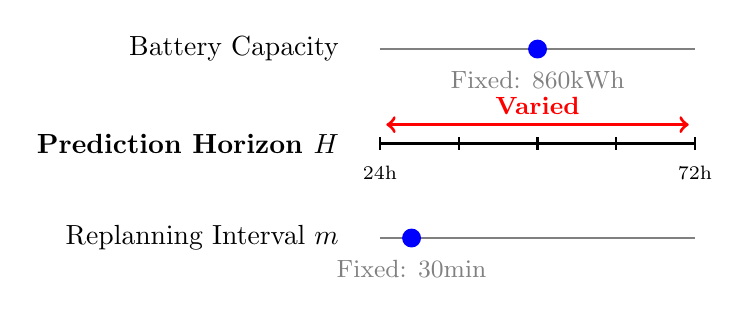
\begin{tikzpicture}[scale=0.8]
    % 蓄電池容量(固定)
    \node[anchor=east] at (-0.5,0) {Battery Capacity};
    \draw[gray, thick] (0,0) -- (5,0);
    \fill[blue] (2.5,0) circle (0.15);
    \node[below, gray] at (2.5,-0.2) {\small Fixed: 860kWh};

    % 予測期間(変化)
    \node[anchor=east] at (-0.5,-1.5) {\textbf{Prediction Horizon $H$}};
    \draw[thick] (0,-1.5) -- (5,-1.5);
    \foreach \x in {0, 1.25, 2.5, 3.75, 5} {
        \draw[thick] (\x,-1.6) -- (\x,-1.4);
    }
    \node[below] at (0,-1.7) {\scriptsize 24h};
    \node[below] at (5,-1.7) {\scriptsize 72h};
    \draw[red, very thick, <->] (0.1,-1.2) -- (4.9,-1.2);
    \node[red, above] at (2.5,-1.2) {\small \textbf{Varied}};

    % 再計画間隔(固定)
    \node[anchor=east] at (-0.5,-3) {Replanning Interval $m$};
    \draw[gray, thick] (0,-3) -- (5,-3);
    \fill[blue] (0.5,-3) circle (0.15);
    \node[below, gray] at (0.5,-3.2) {\small Fixed: 30min};
\end{tikzpicture}
\caption{Comparison axis of this section: prediction horizon $H$ is varied from 24 to 72 hours, while the battery capacity and replanning interval are fixed.}
\label{fig:axis_horizon}
\end{figure}

\subsubsection{予測期間と経済効果}

各予測期間における年間統計をTable~\ref{tab:horizon_comparison}(市場価格連動プラン)およびTable~\ref{tab:horizon_comparison_hokkaido}(北海道電力基本プラン)に示す.

\begin{table}[H]
\centering
\caption{Comparison of annual statistics by prediction horizon (market-linked plan, battery 860\,kWh)}
\label{tab:horizon_comparison}
\begin{tabular}{lrrrr}
\toprule
Item & 24h forecast & 48h forecast & 60h forecast & 72h forecast \\
\midrule
Contract power [kW] & 230.49 & 218.05 & 218.05 & 213.19 \\
Annual purchase [kWh] & 530,742 & 531,358 & 531,418 & 531,373 \\
Annual cost [JPY] & 15,404,698 & 15,023,532 & 15,003,341 & 14,847,956 \\
Cost diff. from 24h [JPY] & - & $-$381,166 & $-$401,357 & $-$556,742 \\
\bottomrule
\end{tabular}
\end{table}

\begin{table}[H]
\centering
\caption{Comparison of annual statistics by prediction horizon (Hokkaido Electric basic plan, battery 860\,kWh)}
\label{tab:horizon_comparison_hokkaido}
\begin{tabular}{lrrrr}
\toprule
Item & 24h forecast & 48h forecast & 60h forecast & 72h forecast \\
\midrule
Contract power [kW] & 169.68 & 166.83 & 166.83 & 166.83 \\
Annual purchase [kWh] & 531,707 & 531,528 & 531,291 & 531,145 \\
Annual cost [JPY] & 14,429,874 & 14,343,827 & 14,339,597 & 14,337,000 \\
Cost diff. from 24h [JPY] & - & $-$86,047 & $-$90,277 & $-$92,874 \\
\bottomrule
\end{tabular}
\end{table}
\noindent
市場価格連動プランでは,予測期間を24時間から48時間に延長することで年間コストが約38.1万円(2.5\%)削減された.60時間予測では48時間予測からわずか約2.0万円の追加削減,72時間予測では48時間予測から約17.6万円の追加削減となり,改善効果の逓減が確認された.

\noindent
北海道電力基本プランでは,予測期間延長による効果がより限定的であり,24時間から72時間への延長で約9.3万円(0.6\%)の削減に留まった.これは,電力量単価が一定のため価格変動への追従が不要であり,主に買電電力の最大値抑制の精度向上のみが効果として現れるためである.

\subsubsection{計算コストとのトレードオフ}

予測期間ごとの計算時間をTable~\ref{tab:horizon_timing}に示す.計算環境はMacBook Pro(Apple M1 Pro, 16GB RAM)である.

\begin{table}[H]
\centering
\caption{Computation time by prediction horizon (battery 860\,kWh)}
\label{tab:horizon_timing}
\begin{tabular}{lrrr}
\toprule
Horizon & Hokkaido [min] & Market [min] & Total [min] \\
\midrule
$H=48$(24時間) & 7.9 & 31.0 & 39.3 \\
$H=96$(48時間) & 16.1 & 16.4 & 33.2 \\
$H=120$(60時間) & 22.7 & 23.2 & 46.3 \\
$H=144$(72時間) & 32.3 & 27.9 & 60.6 \\
\bottomrule
\end{tabular}
\end{table}

\noindent
計算時間は予測期間の延長に伴い概ね増加する傾向が見られた.48時間予測ではコストが約38.1万円削減され,費用対効果が高い.60時間予測は48時間予測から計算時間が約13.1分増加するが,追加のコスト削減はわずか約2.0万円に留まった.本システム構成と検証した4つの予測期間においては,計算資源と削減効果のバランスから48時間(96ステップ)の予測期間が実用的な選択肢の一つであると考えられる.

\subsection{年間一括最適化との比較}

本節では,ローリング計画法の理論的限界を評価するため,年間全データ(17,520ステップ)を一括で最適化するシミュレーションを実施し,その結果をローリング計画法と比較する.年間一括最適化は,将来の需要・PV発電・市場価格を完全に予見した上での理論的最適解であり,ローリング計画法による解がどの程度最適に近いかを評価するベンチマークとなる.

\subsubsection{年間一括最適化の実装}

年間一括最適化では,ローリング計画法と同一の目的関数・制約条件を用いつつ,予測期間$H$を年間全ステップ($H=17{,}520$)に設定した.ただし,目的関数における基本料金項の重み係数$w_{\mathrm{basic}}$は年間按分ではなく,年間の最大買電電力が直接契約電力となるよう式(\ref{eq:weight_basic})において$H = 17{,}520$として計算した.計算時間を1時間に制限したが,すべてのケースで約2分以内に最適解が発見され,制限時間には到達しなかった.

\subsubsection{蓄電池容量別の比較結果}

蓄電池容量430kWh,860kWh,1290kWhの3ケースについて,ローリング計画法(48時間予測)と年間一括最適化の結果を比較した.Table~\ref{tab:annual_vs_rolling_hokkaido}に北海道電力基本プラン,Table~\ref{tab:annual_vs_rolling_market}に市場価格連動プランの結果を示す.

\begin{table}[H]
\centering
\caption{Comparison of rolling horizon and annual batch optimization (Hokkaido Electric basic plan)}
\label{tab:annual_vs_rolling_hokkaido}
\begin{tabular}{lrrrrr}
\toprule
Capacity [kWh] & \multicolumn{2}{c}{Annual Cost [$\times$10k JPY]} & Cost Diff. & \multicolumn{2}{c}{Contract Power [kW]} \\
\cmidrule(lr){2-3} \cmidrule(lr){5-6}
 & Rolling & Annual & [$\times$10k JPY] (\%) & Rolling & Annual \\
\midrule
430 & 1,494.2 & 1,490.0 & $-$4.2 (0.28\%) & 185.5 & 185.5 \\
860 & 1,434.4 & 1,427.8 & $-$6.6 (0.46\%) & 166.8 & 166.8 \\
1290 & 1,407.4 & 1,397.8 & $-$9.6 (0.69\%) & 157.4 & 156.4 \\
\bottomrule
\end{tabular}
\end{table}

\begin{table}[H]
\centering
\caption{Comparison of rolling horizon and annual batch optimization (market-linked plan)}
\label{tab:annual_vs_rolling_market}
\begin{tabular}{lrrrrr}
\toprule
Capacity [kWh] & \multicolumn{2}{c}{Annual Cost [$\times$10k JPY]} & Cost Diff. & \multicolumn{2}{c}{Contract Power [kW]} \\
\cmidrule(lr){2-3} \cmidrule(lr){5-6}
 & Rolling & Annual & [$\times$10k JPY] (\%) & Rolling & Annual \\
\midrule
430 & 1,461.3 & 1,338.9 & $-$122.4 (8.4\%) & 201.4 & 185.5 \\
860 & 1,502.4 & 1,262.9 & $-$239.5 (15.9\%) & 218.1 & 166.8 \\
1290 & 1,512.5 & 1,233.4 & $-$279.1 (18.5\%) & 221.6 & 156.4 \\
\bottomrule
\end{tabular}
\end{table}

\noindent
北海道電力基本プランでは,ローリング計画法と年間一括最適化のコスト差は0.28\%〜0.69\%と小さく,ローリング計画法でもほぼ最適解に近い結果が得られていることが確認された.一方,市場価格連動プランでは8.4\%〜18.5\%と大きな差が生じた.この差異の原因について次節で考察する.

\subsubsection{計算時間の比較}

年間一括最適化の計算時間をTable~\ref{tab:annual_timing}に示す.

\begin{table}[H]
\centering
\caption{Computation time of annual batch optimization}
\label{tab:annual_timing}
\begin{tabular}{lrr}
\toprule
Capacity [kWh] & Hokkaido [min] & Market [min] \\
\midrule
430 & 2.2 & 1.9 \\
860 & 2.0 & 2.5 \\
1290 & 2.6 & 2.2 \\
\bottomrule
\end{tabular}
\end{table}

\noindent
年間一括最適化は約2分で完了し,ローリング計画法(約35〜40分)の約20分の1の計算時間であった.これは,ローリング計画法が17,520回の小規模最適化問題を逐次解くのに対し,年間一括最適化は1回の大規模最適化問題を解くためである.現代のMIPソルバー(SCIP)の効率的な前処理とカット生成により,短時間で最適解が発見された.

\subsubsection{料金プラン優位性の再評価}

年間一括最適化の結果に基づき,料金プランの優位性を再評価した(Table~\ref{tab:plan_comparison_annual}).

\begin{table}[H]
\centering
\caption{Pricing plan comparison using annual batch optimization}
\label{tab:plan_comparison_annual}
\begin{tabular}{lrrrl}
\toprule
Capacity [kWh] & Hokkaido [$\times$10k JPY] & Market [$\times$10k JPY] & Diff. [$\times$10k JPY] & Cheaper Plan \\
\midrule
430 & 1,490.0 & 1,338.9 & $-$151.1 & \textbf{Market} \\
860 & 1,427.8 & 1,262.9 & $-$164.9 & \textbf{Market} \\
1290 & 1,397.8 & 1,233.4 & $-$164.4 & \textbf{Market} \\
\bottomrule
\end{tabular}
\end{table}

\noindent
ローリング計画法では蓄電池容量540kWh以上で北海道電力基本プランが有利となる「優位性逆転」が観察された(Table~\ref{tab:capacity_plan_comparison})が,年間一括最適化では\textbf{全ての容量において市場価格連動プランが有利}という結果となった.この差異は,ローリング計画法における市場価格連動プランの運用が局所最適に陥っていることを示唆する.

\subsubsection{近視眼的最適化による契約電力増大}
\label{sec:bounded_rationality}

前節で明らかになった市場価格連動プランにおけるローリング計画法の性能劣化(年間一括最適化との乖離8~18\%)のメカニズムを分析する.
本研究のローリング計画法におけるコントローラは,48時間という限られた予測期間内でのみ最適化を行う.北海道電力基本プランでは電力量料金が一定(30.56円/kWh)のため,コントローラの局所的最適行動(買電電力の平準化)が自然に大域的最適(契約電力抑制)と一致する.

一方,市場価格連動プランではJEPX価格の変動(3.80~31.00円/kWh)により,コントローラは「安価な時間帯に買電を集中」という局所的に最適な行動をとる.この行動は48時間内では確かに最適だが,年間を通じて繰り返されると,特定の時間帯(深夜帯など)に買電が集中し,契約電力が増大する.

\begin{equation}
\underbrace{\sum_{t \in \mathcal{H}} \pi_t \cdot p_t^{\mathrm{BY}}}_{\text{電力量料金の最小化(局所目標)}} \quad \text{vs.} \quad \underbrace{\max_{t \in \mathcal{Y}} p_t^{\mathrm{BY}}}_{\text{契約電力の抑制(大域目標)}}
\end{equation}

\noindent
ここで$\mathcal{H}$は予測期間,$\mathcal{Y}$は年間全期間である.エージェントは$\mathcal{H}$内での電力量料金最小化を優先するが,この行動が$\mathcal{Y}$における契約電力増大を招く.

特に問題となるのは,蓄電池容量が大きいほど各時点での「安価電力の買いだめ」能力が高まり,契約電力の増大を招くことである.Table~\ref{tab:annual_vs_rolling_market}において,蓄電池容量の増加に伴い契約電力が185.5kW(430kWh)から221.6kW(1290kWh)へと増加した現象は,このメカニズムの発現である.

北海道電力基本プランではこの問題が自然に回避される.電力量料金が時間によらず一定のため,「安価な時間帯への買電集中」というインセンティブが存在しないからである.

\subsection{再計画間隔と長期予測期間の影響}

本節では,蓄電池860kWhの条件下において,\textbf{再計画間隔$m$}および\textbf{予測期間$H$}を変化させた際の影響を検証する(Fig.\ref{fig:axis_interval}).

\begin{figure}[H]
\centering
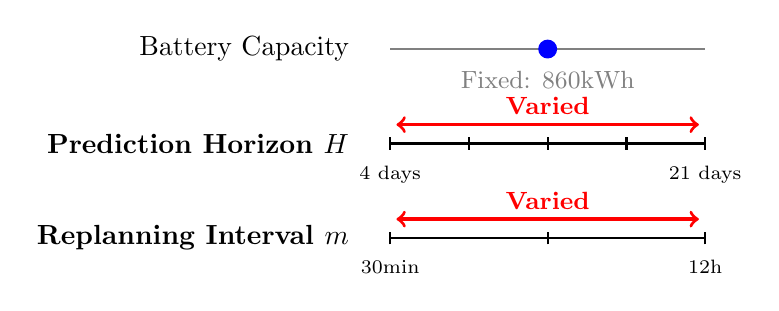
\begin{tikzpicture}[scale=0.8]
    % 蓄電池容量(固定)
    \node[anchor=east] at (-0.5,0) {Battery Capacity};
    \draw[gray, thick] (0,0) -- (5,0);
    \fill[blue] (2.5,0) circle (0.15);
    \node[below, gray] at (2.5,-0.2) {\small Fixed: 860kWh};

    % 予測期間(変化)
    \node[anchor=east] at (-0.5,-1.5) {\textbf{Prediction Horizon $H$}};
    \draw[thick] (0,-1.5) -- (5,-1.5);
    \foreach \x in {0, 1.25, 2.5, 3.75, 5} {
        \draw[thick] (\x,-1.6) -- (\x,-1.4);
    }
    \node[below] at (0,-1.7) {\scriptsize 4 days};
    \node[below] at (5,-1.7) {\scriptsize 21 days};
    \draw[red, very thick, <->] (0.1,-1.2) -- (4.9,-1.2);
    \node[red, above] at (2.5,-1.2) {\small \textbf{Varied}};

    % 再計画間隔(変化)
    \node[anchor=east] at (-0.5,-3) {\textbf{Replanning Interval $m$}};
    \draw[thick] (0,-3) -- (5,-3);
    \foreach \x in {0, 2.5, 5} {
        \draw[thick] (\x,-3.1) -- (\x,-2.9);
    }
    \node[below] at (0,-3.2) {\scriptsize 30min};
    \node[below] at (5,-3.2) {\scriptsize 12h};
    \draw[red, very thick, <->] (0.1,-2.7) -- (4.9,-2.7);
    \node[red, above] at (2.5,-2.7) {\small \textbf{Varied}};
\end{tikzpicture}
\caption{Comparison axes of this section: both the prediction horizon $H$ (4--21 days) and replanning interval $m$ (30\,min--12\,h) are varied.}
\label{fig:axis_interval}
\end{figure}

\subsubsection{再計画間隔の影響}

予測期間96ステップ(48時間)において,再計画間隔(Replan. Interval)を変化させた結果をTable~\ref{tab:control_horizon}に示す.表中のComp. Timeは計算時間,Time Reductionは計算時間の削減率を表す.

\begin{table}[H]
\centering
\caption{Effect of replanning interval (prediction horizon 48\,h, battery 860\,kWh)}
\label{tab:control_horizon}
\begin{tabular}{lrrrr}
\toprule
Replan. Interval & Hokkaido [$\times$10k JPY] & Market [$\times$10k JPY] & Comp. Time [min] & Time Reduction \\
\midrule
1 step (30 min) & 1,434.4 & 1,502.4 & 33.2 & - \\
2 steps (1 hour) & 1,434.4 & 1,502.2 & 15.9 & 52\% \\
4 steps (2 hours) & 1,434.4 & 1,501.6 & 7.9 & 76\% \\
8 steps (4 hours) & 1,434.4 & 1,500.7 & 4.1 & 88\% \\
\bottomrule
\end{tabular}
\end{table}

\noindent
北海道電力基本プランではコストへの影響がなく,市場価格連動プランでも最大0.1\%程度の差に留まった.一方,計算時間は再計画間隔8で基準の約\textbf{12\%}まで短縮された.この結果は,再計画間隔の延長が計算効率の大幅な改善をもたらす一方,解の品質への影響は限定的であることを示す.

\subsubsection{長期予測期間と再計画間隔の組み合わせ}

再計画間隔の延長により計算時間を抑制しつつ,予測期間を192ステップ(4日間),384ステップ(8日間),672ステップ(14日間)まで延長した結果をTable~\ref{tab:long_horizon}に示す.

\begin{table}[H]
\centering
\small
\caption{Effect of long-term prediction horizon and replanning interval (battery 860\,kWh)}
\label{tab:long_horizon}
\begin{tabular}{llrrrr}
\toprule
Horizon & Control $m$ & Hokkaido [$\times$10k JPY] & Market [$\times$10k JPY] & Comp. Time [min] & vs. Annual \\
\midrule
24h (48) & 1 & 1,443.0 & 1,540.5 & 39.3 & 22.0\% \\
48h (96) & 1 & 1,434.4 & 1,502.4 & 33.2 & 19.0\% \\
\midrule
4 days (192) & 2 & 1,433.1 & 1,452.7 & 46.4 & 15.0\% \\
4 days (192) & 4 & 1,433.1 & 1,452.5 & 23.1 & 15.0\% \\
4 days (192) & 8 & 1,433.1 & 1,448.3 & 11.1 & 14.7\% \\
\midrule
8 days (384) & 4 & 1,431.5 & 1,420.9 & 53.1 & 12.5\% \\
8 days (384) & 8 & 1,431.5 & 1,420.6 & 25.5 & 12.5\% \\
\midrule
14 days (672) & 8 & 1,430.4 & 1,398.9 & 48.5 & 10.8\% \\
14 days (672) & 16 & 1,430.4 & 1,398.8 & 25.1 & 10.8\% \\
\midrule
21 days (1008) & 24 & 1,429.9 & 1,380.2 & 27.6 & 9.3\% \\
\midrule
\multicolumn{2}{l}{Annual batch} & 1,427.8 & 1,262.9 & 4.5 & 0\% \\
\bottomrule
\end{tabular}
\end{table}

\noindent
「年間一括比」は市場価格連動プランにおいて,年間一括最適化との差を示す($(コスト - 1262.9) / 1262.9 \times 100$).

これらの結果から,予測期間延長の効果と計算効率のトレードオフについて重要な知見が得られた.

まず予測期間延長の効果について,予測期間を14日間(672ステップ)まで延長することで,市場価格連動プランのコストは1,398.9万円まで改善し,年間一括最適化との差は22.0\%から10.8\%まで縮小した.この改善は,長期予測により将来の価格変動を見越した運用が可能となり,契約電力の増大を抑制できたためと考えられる.

さらに注目すべきは,8日間(384ステップ)以上の予測期間では,市場価格連動プラン(1,420.9万円)が北海道電力基本プラン(1,431.5万円)より10.6万円安価となり,年間一括最適化と同様に市場連動プランの優位性が回復した点である.この結果は,48時間予測で観察された「蓄電池容量増加に伴う市場連動プランの不利化」が,予測期間の制約に起因する局所最適の問題であったことを示唆している.

計算コストの観点からは,再計画間隔8を用いることで,14日間予測でも計算時間を48.5分に抑制できることが確認された.これは48時間予測・再計画間隔1(33.2分)と同程度であり,実用的な計算時間の範囲内である.また,同一予測期間では,再計画間隔によるコスト差は0.5万円未満に留まり,計算効率の改善効果が支配的であった.したがって,再計画間隔の延長は解の品質をほぼ維持しながら計算時間を大幅に短縮する有効な手法である.


\subsection{予測の不確実性に対する頑健性}
\label{sec:robustness}

本研究のシミュレーションは完全予見(Perfect Forecast)を前提としている.しかし,実運用では予測誤差が不可避であり,その影響を定性的に考察する.

ローリング計画法はフィードバック制御構造を持つため,需要誤差などの可逆的な変動に対しては一定の自己修正能力を有する.一方,契約電力の決定要因となる最大買電電力は不可逆的な指標であり,一度でも高い値を記録すると修正が効かない.

この観点から料金プランを比較すると,北海道電力基本プランは電力量単価が一定であり,買電平準化が常に最適となるため,予測誤差に対して比較的頑健である.対して市場価格連動プランは,価格差を利用した時間的裁定を行うため,価格予測誤差による損失や,意図せぬピーク発生リスクに対して脆弱である.

したがって,予測誤差が存在する実環境においては,市場価格連動プランの優位性が低下し,北海道電力基本プランの安定性が相対的に高まると考えられる.本研究の「北海道電力基本プラン+大容量蓄電池が有利」という結論は,実運用環境においても妥当性を持つ可能性が高い.


\subsection{モデルの制約と限界}
\label{sec:wbasic_limitation}

本節では,採用した最適化手法の限界と,それが結果に与える影響を明確にする.

\subsubsection{基本料金係数の按分手法}

契約電力(基本料金の決定要因)は,本来「年間17,520ステップの中の最大買電電力」という\textbf{大域的な指標}で決定される.しかし,ローリング計画法では年間を通した最適化が計算上困難であるため,各予測期間(96ステップ,48時間)内の最大値$s^{\mathrm{BY}}_{\mathrm{MAX}}$に按分係数$w_{\mathrm{basic}}$を乗じてペナルティを与える近似を採用した.

この「局所的な最大値の抑制」を通じて「大域的な最大値」を間接的に制御する手法には,いくつかの数理的問題がある.

まず,最適化基準と評価基準に乖離が存在する.ソルバーは各予測期間で「$w_{\mathrm{basic}} \times s^{\mathrm{BY}}_{\mathrm{MAX}}$」を最小化しようとするが,最終的な基本料金は「年間最大買電電力 × 単価」で計算される.この乖離により,局所的な最適化が必ずしも大域的な最適解を与えるとは限らない.

次に,局所最適と大域最適の不一致が問題となる.ある予測期間で買電電力の最大値を抑制する努力が,別の期間で発生するより大きな買電電力により無効化される可能性がある.この問題は,年間を通じた需要パターンに大きな季節変動がある本研究の対象施設において特に顕著となりうる.

さらに,按分係数$w_{\mathrm{basic}}$の値によって,ソルバーの「買電電力の最大値抑制」と「電力量料金削減」のトレードオフ判断が変化する.係数の設定は本質的に経験的であり,最適な値は対象システムや運用条件に依存する.

北海道電力基本プランでは電力量料金が一定であるため,ソルバーは自然に買電電力を平準化する方向に最適化を行い,按分手法の影響は限定的である.一方,市場価格連動プランではJEPX価格の変動(3.80〜31.00円/kWh)により,「安価な時間帯への買電集中」と「買電電力の最大値抑制」のトレードオフが生じ,大容量蓄電池ほど契約電力が増大する傾向が確認された.

\noindent
\textbf{今後の課題}:按分手法の限界を克服するためには,$w_{\mathrm{basic}}$の感度分析,年間契約電力の明示的追跡機構の導入,異なる最適化手法との比較検証が必要である.

\subsubsection{リスクの偏在性と認識の非対称性}
\label{sec:risk_asymmetry}

前節では按分手法の数理的問題を述べたが,本節ではより本質的な問題として「リスクの偏在性」と「認識の非対称性」について論じる.これらの概念は,第\ref{sec:bounded_rationality}節で述べた近視眼的最適化の議論を補完し,市場価格連動プランにおける契約電力増大のメカニズムを理解する上で重要な要因となる.

\noindent\textbf{リスクの時間的偏在性}:

本研究で採用した按分係数$w_{\mathrm{basic}}$は,式(\ref{eq:weight_basic})に示す通り,年間を通じて均等に配分されている:

\begin{equation}
w_{\mathrm{basic}} = \frac{\text{基本料金単価} \times H}{17{,}520} = \frac{1989.0 \times 96}{17{,}520} \approx 10.90 \text{ [円/kW]}
\end{equation}

\noindent
この均等配分は,「年間最大買電電力はいつ発生するか分からない」という不確実性への素朴な対応である.しかし,実際のリスク(年間最大買電電力の発生確率)は時間的に均等ではない.

Fig.\ref{fig:monthly_analysis}に示した月別需要パターンから明らかなように,本研究の対象施設では7月・8月の夏季に需要が集中し,特に8月に年間最大買電電力166.8kWを記録した.すなわち,「年間最大買電電力の発生リスク」は夏季の特定期間に偏在している.

均等配分の$w_{\mathrm{basic}}$は,この偏在性を反映していない.結果として,リスクの低い時期(冬季)には過剰なペナルティを,リスクの高い時期(夏季)には不十分なペナルティを課すことになる.

\noindent\textbf{認識の非対称性}:

より根本的な問題は,ローリング計画法のエージェントが「今こそが年間最大需要の瞬間である」と認識するメカニズムを持たないことである.

人間の意思決定者であれば,以下の情報を総合して「今日は特に注意が必要」と判断できる:

\begin{itemize}
    \item 過去の経験:「去年も1月上旬が最も需要が高かった」
    \item 気象情報:「明日は今季最強の寒波が到来」
    \item 文脈情報:「今日は大型イベント開催で施設稼働率が最大」
\end{itemize}

一方,本研究のエージェントは48時間の予測期間内のデータのみを参照し,以下の認識の非対称性を抱えている:

\begin{equation}
\underbrace{\text{エージェントの視野}}_{\mathcal{H}: \text{48時間}} \ll \underbrace{\text{リスク評価に必要な視野}}_{\mathcal{Y}: \text{年間}}
\end{equation}

この認識の非対称性により,エージェントは各予測期間において「自分の行動が年間最大買電電力を決定してしまうかもしれない」という危機感を持つことができない.特に市場価格連動プランでは,安価な時間帯が出現するたびに,エージェントは「この機会を逃すまい」と貪欲に買電を行う.その結果,年間を通じて散発的に発生する「安価だが大量買電」のエピソードのうち,最も大きなものが契約電力を決定することになる.

\subsubsection{結論の解釈における注意点}

本研究の結論を解釈する際には,以下の点に注意が必要である.まず,予測期間48時間,再計画間隔30分の条件下での市場価格連動プランの「最適容量430kWh」は按分係数の設定値に依存する可能性がある.按分係数を変更することで,最適容量も変化しうる.次に,契約電力の増加現象については,時間的裁定の本質的特性と按分手法の限界の両方が寄与していると考えられる.すなわち,この現象は純粋に物理的な制約によるものではなく,最適化手法の限界も一因となっている可能性がある.最後に,両プラン比較において按分手法の影響に非対称性がある点も重要である.北海道電力基本プランは按分手法の影響を受けにくいのに対し,市場価格連動プランはその影響を強く受けるため,両プランの公平な比較には慎重な解釈が求められる.

\noindent\textbf{改善への示唆}:

リスクの偏在性と認識の非対称性を克服するためのアプローチとして,以下が考えられる:

\begin{itemize}
    \item \textbf{季節別$w_{\mathrm{basic}}$}:冬季には高い$w_{\mathrm{basic}}$,夏季には低い$w_{\mathrm{basic}}$を設定
    \item \textbf{動的$w_{\mathrm{basic}}$}:予測需要が一定閾値を超えた場合に$w_{\mathrm{basic}}$を増大
    \item \textbf{契約電力追跡機構}:現時点までの最大買電電力を状態変数として保持し,それを超える買電に対してのみペナルティを課す
    \item \textbf{確率的定式化}:年間最大需要の発生確率分布を推定し,期待値最小化に基づく最適化
\end{itemize}

これらのアプローチは,エージェントに「大域的視野」を擬似的に付与する試みと解釈できる.ただし,いずれも追加的な計算コストや調整パラメータの導入を伴うため,実装上の課題は残る.

\subsection{一般化可能性と適用範囲}

本研究の結論は,以下の特定条件に依存しており,異なる条件下では結論が変化する可能性がある:

\begin{itemize}
    \item \textbf{対象期間}:2024年1月〜12月のJEPX北海道エリア価格(年間平均16.87円/kWh)
    \item \textbf{地域}:北海道エリア(冬季暖房需要が顕著,本州との連系線容量が限定的)
    \item \textbf{需要特性}:年間812,982kWh,最大電力264.0kW,PV自給率35.4\%
    \item \textbf{システム構成}:PV 250kW,蓄電池出力400kW,系統への電力逆流不可
\end{itemize}

他の電力エリア,異なる年度の市場価格,異なる需要パターン(オフィスビル,工場等),または系統への電力逆流が可能なシステム構成では,最適な料金プランや蓄電池容量が変化する.

ただし,本研究から以下の\textbf{定性的知見}が得られた:

\begin{enumerate}
    \item 料金プランの有利性は蓄電池容量に依存し,逆転する分岐点が存在しうる(予測期間48時間の場合)
    \item 固定価格プランでは契約電力の抑制,変動価格プランでは時間的裁定が最適化の主軸となる
    \item 蓄電池効果は季節により大きく変動する
\end{enumerate}

異なる条件下での最適解を求めるには,本研究で開発した最適化フレームワークに対象地域の市場価格データ,料金体系,需要パターンを入力して再計算する必要がある.

\section{結論}

本研究では,北海道十勝地方のPV・蓄電池システム(PV容量250kW)を対象に,ローリング計画法による運用最適化シミュレーションを実施した.3つの比較軸(蓄電池容量・予測期間・再計画間隔)に沿って体系的に検証し,以下の知見を得た.

\begin{enumerate}
    \item \textbf{蓄電池容量の影響}:予測期間48時間,再計画間隔30分の条件下では,蓄電池容量430kWh以下では市場価格連動プランが有利であるが,540kWh以上では北海道電力基本プランが有利となり,プラン優位性が逆転した.

    \item \textbf{予測期間の影響}:予測期間の延長はコスト削減に寄与する.市場価格連動プランでは8日間以上の長期予測により優位性が回復し,21日間予測では両プランがほぼ同等となった.

    \item \textbf{再計画間隔の影響}:再計画間隔を4時間に延長することで計算時間を約88\%削減しつつ,コストへの影響は0.5万円未満に抑制できた.

    \item \textbf{年間一括最適化との比較}:北海道電力基本プランではローリング計画法でもほぼ最適解(コスト差0.3~0.7\%)を達成するが,市場価格連動プランでは予測期間48時間,再計画間隔30分の条件下で8~18\%のコスト差が生じた.長期予測によりこの差は縮小する.

    \item \textbf{条件依存性}:料金プランの優位性は蓄電池容量と予測期間の両方に依存し,単一の「最適プラン」は存在しない.実用上は,予測可能な期間と計算資源を考慮した上で,適切な運用パラメータを選択する必要がある.
\end{enumerate}

\section*{謝辞}
\addcontentsline{toc}{section}{謝辞}

本研究を進めるにあたり,終始丁寧なご指導を賜りました玉置久教授に心より感謝申し上げます.
また,研究の進め方についてご助言をいただきました森田紘平特命助教に深く感謝いたします.
さらに,日頃より研究に関する議論や助言をいただきました同研究室修士2年の奥村侑真氏に厚く御礼申し上げます.

\begin{thebibliography}{99}
\addcontentsline{toc}{section}{参考文献}
  \bibitem{scip}
  SCIP: Solving Constraint Integer Programs, \url{https://www.scipopt.org/}

  \bibitem{jepx}
  日本卸電力取引所(JEPX), \url{https://www.jepx.jp/electricpower/market-data/spot/}
\end{thebibliography}

\end{document}
